\documentclass[sigconf,nonacm]{acmart}

\usepackage{booktabs}
\usepackage{tabularx}
\usepackage{xspace}
\usepackage[capitalise,noabbrev]{cleveref}

\settopmatter{printacmref=false,printccs=false,printfolios=true}
\renewcommand\footnotetextcopyrightpermission[1]{}
\pagestyle{plain}

\setlength{\emergencystretch}{2.5em}
\newcommand{\hstore}{HStore\xspace}
\newcommand{\hgdb}{HyperGraphDB\xspace}
\newcommand{\wl}[1]{\textsf{#1}}
\newcommand{\code}[1]{\texttt{#1}}
\makeatletter
\newcommand{\M}[1]{\@ifundefined{m@#1}{\textbf{??#1}}{\csname m@#1\endcsname}}
\expandafter\def\csname m@ratios1asyncingestnodes\endcsname{1.7}
\expandafter\def\csname m@hss1asyncingestnodes\endcsname{33.3\,k}
\expandafter\def\csname m@hgs1asyncingestnodes\endcsname{19.6\,k}
\expandafter\def\csname m@ratios1asyncingestedges\endcsname{1.4}
\expandafter\def\csname m@hss1asyncingestedges\endcsname{28.9\,k}
\expandafter\def\csname m@hgs1asyncingestedges\endcsname{21.3\,k}
\expandafter\def\csname m@ratios1asyncreadincidence\endcsname{2.5}
\expandafter\def\csname m@hss1asyncreadincidence\endcsname{3.10\,M}
\expandafter\def\csname m@hgs1asyncreadincidence\endcsname{1.25\,M}
\expandafter\def\csname m@ratios1asyncreadmembers\endcsname{1.4}
\expandafter\def\csname m@hss1asyncreadmembers\endcsname{2.29\,M}
\expandafter\def\csname m@hgs1asyncreadmembers\endcsname{1.66\,M}
\expandafter\def\csname m@ratios1asyncreadcomembership\endcsname{5.5}
\expandafter\def\csname m@hss1asyncreadcomembership\endcsname{272\,k}
\expandafter\def\csname m@hgs1asyncreadcomembership\endcsname{49.8\,k}
\expandafter\def\csname m@ratios1asyncreadtwohop\endcsname{2.9}
\expandafter\def\csname m@hss1asyncreadtwohop\endcsname{243\,k}
\expandafter\def\csname m@hgs1asyncreadtwohop\endcsname{83.6\,k}
\expandafter\def\csname m@ratios1asyncreadincidenceparallel\endcsname{11}
\expandafter\def\csname m@hss1asyncreadincidenceparallel\endcsname{14.1\,M}
\expandafter\def\csname m@hgs1asyncreadincidenceparallel\endcsname{1.28\,M}
\expandafter\def\csname m@ratios1asynclatencyread\endcsname{4.1}
\expandafter\def\csname m@hss1asynclatencyread\endcsname{2.07\,M}
\expandafter\def\csname m@hgs1asynclatencyread\endcsname{505\,k}
\expandafter\def\csname m@ratios1asyncwriteupdate\endcsname{5.6}
\expandafter\def\csname m@hss1asyncwriteupdate\endcsname{40.9\,k}
\expandafter\def\csname m@hgs1asyncwriteupdate\endcsname{7.26\,k}
\expandafter\def\csname m@ratios1asynclatencycommit\endcsname{0.95$^\dagger$}
\expandafter\def\csname m@hss1asynclatencycommit\endcsname{6.96\,k}
\expandafter\def\csname m@hgs1asynclatencycommit\endcsname{7.33\,k}
\expandafter\def\csname m@ratios1asyncmixedread\endcsname{7.7}
\expandafter\def\csname m@hss1asyncmixedread\endcsname{8.73\,M}
\expandafter\def\csname m@hgs1asyncmixedread\endcsname{1.13\,M}
\expandafter\def\csname m@ratios1asyncmixedwrite\endcsname{1.0}
\expandafter\def\csname m@hss1asyncmixedwrite\endcsname{1,000}
\expandafter\def\csname m@hgs1asyncmixedwrite\endcsname{1,000}
\expandafter\def\csname m@ratios1asynclargeingest\endcsname{9.1}
\expandafter\def\csname m@hss1asynclargeingest\endcsname{431\,k}
\expandafter\def\csname m@hgs1asynclargeingest\endcsname{47.6\,k}
\expandafter\def\csname m@ratios1asynclargescan\endcsname{4.8}
\expandafter\def\csname m@hss1asynclargescan\endcsname{1,668\,M}
\expandafter\def\csname m@hgs1asynclargescan\endcsname{344\,M}
\expandafter\def\csname m@ratios1asynclargeprobe\endcsname{6.5}
\expandafter\def\csname m@hss1asynclargeprobe\endcsname{6.60\,M}
\expandafter\def\csname m@hgs1asynclargeprobe\endcsname{1.01\,M}
\expandafter\def\csname m@ratios1asyncreopen\endcsname{12.5}
\expandafter\def\csname m@hss1asyncreopen\endcsname{78.5\,ms}
\expandafter\def\csname m@hgs1asyncreopen\endcsname{978\,ms}
\expandafter\def\csname m@ratios1asyncreadincidencecold\endcsname{25.6}
\expandafter\def\csname m@hss1asyncreadincidencecold\endcsname{1.73\,M}
\expandafter\def\csname m@hgs1asyncreadincidencecold\endcsname{67.6\,k}
\expandafter\def\csname m@ratios1asyncdisk\endcsname{4.7}
\expandafter\def\csname m@hss1asyncdisk\endcsname{85.7\,MiB}
\expandafter\def\csname m@hgs1asyncdisk\endcsname{400\,MiB}
\expandafter\def\csname m@ratios1asyncchurndelete\endcsname{3.1}
\expandafter\def\csname m@hss1asyncchurndelete\endcsname{16.1\,k}
\expandafter\def\csname m@hgs1asyncchurndelete\endcsname{5.18\,k}
\expandafter\def\csname m@ratios1asyncchurnremove\endcsname{2.2}
\expandafter\def\csname m@hss1asyncchurnremove\endcsname{23.1\,k}
\expandafter\def\csname m@hgs1asyncchurnremove\endcsname{10.7\,k}
\expandafter\def\csname m@ratios1asyncreadincidencechurned\endcsname{2.4}
\expandafter\def\csname m@hss1asyncreadincidencechurned\endcsname{3.10\,M}
\expandafter\def\csname m@hgs1asyncreadincidencechurned\endcsname{1.30\,M}
\expandafter\def\csname m@ratios1asyncdiskchurned\endcsname{2.5}
\expandafter\def\csname m@hss1asyncdiskchurned\endcsname{116\,MiB}
\expandafter\def\csname m@hgs1asyncdiskchurned\endcsname{293\,MiB}
\expandafter\def\csname m@ratios1asynccompactionbaseline\endcsname{1.0$^\dagger$}
\expandafter\def\csname m@hss1asynccompactionbaseline\endcsname{50.1}
\expandafter\def\csname m@hgs1asynccompactionbaseline\endcsname{50.1}
\expandafter\def\csname m@ratios1asynccompaction\endcsname{1.0$^\dagger$}
\expandafter\def\csname m@hss1asynccompaction\endcsname{50.1}
\expandafter\def\csname m@hgs1asynccompaction\endcsname{50.1}
\expandafter\def\csname m@ratios1asyncdiskcompacted\endcsname{2.5}
\expandafter\def\csname m@hss1asyncdiskcompacted\endcsname{93.3\,MiB}
\expandafter\def\csname m@hgs1asyncdiskcompacted\endcsname{234\,MiB}
\expandafter\def\csname m@ratios1asyncrecover\endcsname{1.3$^\dagger$}
\expandafter\def\csname m@hss1asyncrecover\endcsname{84.8\,ms}
\expandafter\def\csname m@hgs1asyncrecover\endcsname{113\,ms}
\expandafter\def\csname m@ratios1syncingestnodes\endcsname{1.7}
\expandafter\def\csname m@hss1syncingestnodes\endcsname{33.9\,k}
\expandafter\def\csname m@hgs1syncingestnodes\endcsname{19.6\,k}
\expandafter\def\csname m@ratios1syncingestedges\endcsname{1.3}
\expandafter\def\csname m@hss1syncingestedges\endcsname{27.8\,k}
\expandafter\def\csname m@hgs1syncingestedges\endcsname{20.8\,k}
\expandafter\def\csname m@ratios1syncreadincidence\endcsname{3.1}
\expandafter\def\csname m@hss1syncreadincidence\endcsname{3.71\,M}
\expandafter\def\csname m@hgs1syncreadincidence\endcsname{1.18\,M}
\expandafter\def\csname m@ratios1syncreadmembers\endcsname{1.6}
\expandafter\def\csname m@hss1syncreadmembers\endcsname{2.45\,M}
\expandafter\def\csname m@hgs1syncreadmembers\endcsname{1.58\,M}
\expandafter\def\csname m@ratios1syncreadcomembership\endcsname{4.9}
\expandafter\def\csname m@hss1syncreadcomembership\endcsname{281\,k}
\expandafter\def\csname m@hgs1syncreadcomembership\endcsname{57.8\,k}
\expandafter\def\csname m@ratios1syncreadtwohop\endcsname{3.4}
\expandafter\def\csname m@hss1syncreadtwohop\endcsname{257\,k}
\expandafter\def\csname m@hgs1syncreadtwohop\endcsname{75.7\,k}
\expandafter\def\csname m@ratios1syncreadincidenceparallel\endcsname{12.8}
\expandafter\def\csname m@hss1syncreadincidenceparallel\endcsname{16.8\,M}
\expandafter\def\csname m@hgs1syncreadincidenceparallel\endcsname{1.32\,M}
\expandafter\def\csname m@ratios1synclatencyread\endcsname{3.8}
\expandafter\def\csname m@hss1synclatencyread\endcsname{2.21\,M}
\expandafter\def\csname m@hgs1synclatencyread\endcsname{575\,k}
\expandafter\def\csname m@ratios1syncwriteupdate\endcsname{5.8}
\expandafter\def\csname m@hss1syncwriteupdate\endcsname{41.6\,k}
\expandafter\def\csname m@hgs1syncwriteupdate\endcsname{7.22\,k}
\expandafter\def\csname m@ratios1synclatencycommit\endcsname{1.2}
\expandafter\def\csname m@hss1synclatencycommit\endcsname{1.78\,k}
\expandafter\def\csname m@hgs1synclatencycommit\endcsname{1.44\,k}
\expandafter\def\csname m@ratios1syncmixedread\endcsname{8.0}
\expandafter\def\csname m@hss1syncmixedread\endcsname{9.12\,M}
\expandafter\def\csname m@hgs1syncmixedread\endcsname{1.14\,M}
\expandafter\def\csname m@ratios1syncmixedwrite\endcsname{1.0}
\expandafter\def\csname m@hss1syncmixedwrite\endcsname{1,000}
\expandafter\def\csname m@hgs1syncmixedwrite\endcsname{1,000}
\expandafter\def\csname m@ratios1synclargeingest\endcsname{7.4}
\expandafter\def\csname m@hss1synclargeingest\endcsname{411\,k}
\expandafter\def\csname m@hgs1synclargeingest\endcsname{55.8\,k}
\expandafter\def\csname m@ratios1synclargescan\endcsname{4.5}
\expandafter\def\csname m@hss1synclargescan\endcsname{1,669\,M}
\expandafter\def\csname m@hgs1synclargescan\endcsname{375\,M}
\expandafter\def\csname m@ratios1synclargeprobe\endcsname{7.2}
\expandafter\def\csname m@hss1synclargeprobe\endcsname{6.62\,M}
\expandafter\def\csname m@hgs1synclargeprobe\endcsname{923\,k}
\expandafter\def\csname m@ratios1syncreopen\endcsname{13}
\expandafter\def\csname m@hss1syncreopen\endcsname{80.4\,ms}
\expandafter\def\csname m@hgs1syncreopen\endcsname{1,044\,ms}
\expandafter\def\csname m@ratios1syncreadincidencecold\endcsname{28.1}
\expandafter\def\csname m@hss1syncreadincidencecold\endcsname{1.95\,M}
\expandafter\def\csname m@hgs1syncreadincidencecold\endcsname{69.2\,k}
\expandafter\def\csname m@ratios1syncdisk\endcsname{4.3}
\expandafter\def\csname m@hss1syncdisk\endcsname{85.8\,MiB}
\expandafter\def\csname m@hgs1syncdisk\endcsname{371\,MiB}
\expandafter\def\csname m@ratios1syncchurndelete\endcsname{2.9}
\expandafter\def\csname m@hss1syncchurndelete\endcsname{16.3\,k}
\expandafter\def\csname m@hgs1syncchurndelete\endcsname{5.67\,k}
\expandafter\def\csname m@ratios1syncchurnremove\endcsname{2.1}
\expandafter\def\csname m@hss1syncchurnremove\endcsname{23.6\,k}
\expandafter\def\csname m@hgs1syncchurnremove\endcsname{11.3\,k}
\expandafter\def\csname m@ratios1syncreadincidencechurned\endcsname{2.6}
\expandafter\def\csname m@hss1syncreadincidencechurned\endcsname{3.44\,M}
\expandafter\def\csname m@hgs1syncreadincidencechurned\endcsname{1.30\,M}
\expandafter\def\csname m@ratios1syncdiskchurned\endcsname{2.0}
\expandafter\def\csname m@hss1syncdiskchurned\endcsname{118\,MiB}
\expandafter\def\csname m@hgs1syncdiskchurned\endcsname{234\,MiB}
\expandafter\def\csname m@ratios1synccompactionbaseline\endcsname{1.0$^\dagger$}
\expandafter\def\csname m@hss1synccompactionbaseline\endcsname{50.1}
\expandafter\def\csname m@hgs1synccompactionbaseline\endcsname{50.1}
\expandafter\def\csname m@ratios1synccompaction\endcsname{1.0$^\dagger$}
\expandafter\def\csname m@hss1synccompaction\endcsname{50.1}
\expandafter\def\csname m@hgs1synccompaction\endcsname{50.1}
\expandafter\def\csname m@ratios1syncdiskcompacted\endcsname{2.7}
\expandafter\def\csname m@hss1syncdiskcompacted\endcsname{93.3\,MiB}
\expandafter\def\csname m@hgs1syncdiskcompacted\endcsname{254\,MiB}
\expandafter\def\csname m@ratios1syncrecover\endcsname{1.4}
\expandafter\def\csname m@hss1syncrecover\endcsname{77.7\,ms}
\expandafter\def\csname m@hgs1syncrecover\endcsname{111\,ms}
\expandafter\def\csname m@ratios4asyncingestnodes\endcsname{1.8}
\expandafter\def\csname m@hss4asyncingestnodes\endcsname{42.9\,k}
\expandafter\def\csname m@hgs4asyncingestnodes\endcsname{24.0\,k}
\expandafter\def\csname m@ratios4asyncingestedges\endcsname{7.9}
\expandafter\def\csname m@hss4asyncingestedges\endcsname{21.5\,k}
\expandafter\def\csname m@hgs4asyncingestedges\endcsname{2.71\,k}
\expandafter\def\csname m@ratios4asyncreadincidence\endcsname{2.4}
\expandafter\def\csname m@hss4asyncreadincidence\endcsname{2.62\,M}
\expandafter\def\csname m@hgs4asyncreadincidence\endcsname{1.11\,M}
\expandafter\def\csname m@ratios4asyncreadmembers\endcsname{1.7}
\expandafter\def\csname m@hss4asyncreadmembers\endcsname{2.13\,M}
\expandafter\def\csname m@hgs4asyncreadmembers\endcsname{1.27\,M}
\expandafter\def\csname m@ratios4asyncreadcomembership\endcsname{6.8}
\expandafter\def\csname m@hss4asyncreadcomembership\endcsname{281\,k}
\expandafter\def\csname m@hgs4asyncreadcomembership\endcsname{41.4\,k}
\expandafter\def\csname m@ratios4asyncreadtwohop\endcsname{2.1}
\expandafter\def\csname m@hss4asyncreadtwohop\endcsname{172\,k}
\expandafter\def\csname m@hgs4asyncreadtwohop\endcsname{80.9\,k}
\expandafter\def\csname m@ratios4asyncreadincidenceparallel\endcsname{6.5}
\expandafter\def\csname m@hss4asyncreadincidenceparallel\endcsname{8.21\,M}
\expandafter\def\csname m@hgs4asyncreadincidenceparallel\endcsname{1.26\,M}
\expandafter\def\csname m@ratios4asynclatencyread\endcsname{3.8}
\expandafter\def\csname m@hss4asynclatencyread\endcsname{1.79\,M}
\expandafter\def\csname m@hgs4asynclatencyread\endcsname{470\,k}
\expandafter\def\csname m@ratios4asyncwriteupdate\endcsname{12.2}
\expandafter\def\csname m@hss4asyncwriteupdate\endcsname{30.2\,k}
\expandafter\def\csname m@hgs4asyncwriteupdate\endcsname{2.47\,k}
\expandafter\def\csname m@ratios4asynclatencycommit\endcsname{4.0}
\expandafter\def\csname m@hss4asynclatencycommit\endcsname{10.1\,k}
\expandafter\def\csname m@hgs4asynclatencycommit\endcsname{2.54\,k}
\expandafter\def\csname m@ratios4asyncmixedread\endcsname{7.7}
\expandafter\def\csname m@hss4asyncmixedread\endcsname{8.55\,M}
\expandafter\def\csname m@hgs4asyncmixedread\endcsname{1.11\,M}
\expandafter\def\csname m@ratios4asyncmixedwrite\endcsname{1.0}
\expandafter\def\csname m@hss4asyncmixedwrite\endcsname{1,000}
\expandafter\def\csname m@hgs4asyncmixedwrite\endcsname{999}
\expandafter\def\csname m@ratios4asynclargeingest\endcsname{36.1}
\expandafter\def\csname m@hss4asynclargeingest\endcsname{489\,k}
\expandafter\def\csname m@hgs4asynclargeingest\endcsname{13.6\,k}
\expandafter\def\csname m@ratios4asynclargescan\endcsname{4.4}
\expandafter\def\csname m@hss4asynclargescan\endcsname{1,583\,M}
\expandafter\def\csname m@hgs4asynclargescan\endcsname{358\,M}
\expandafter\def\csname m@ratios4asynclargeprobe\endcsname{6.7}
\expandafter\def\csname m@hss4asynclargeprobe\endcsname{5.61\,M}
\expandafter\def\csname m@hgs4asynclargeprobe\endcsname{844\,k}
\expandafter\def\csname m@ratios4asyncreopen\endcsname{13.8}
\expandafter\def\csname m@hss4asyncreopen\endcsname{92.9\,ms}
\expandafter\def\csname m@hgs4asyncreopen\endcsname{1,279\,ms}
\expandafter\def\csname m@ratios4asyncreadincidencecold\endcsname{81.6}
\expandafter\def\csname m@hss4asyncreadincidencecold\endcsname{1.23\,M}
\expandafter\def\csname m@hgs4asyncreadincidencecold\endcsname{15.1\,k}
\expandafter\def\csname m@ratios4asyncdisk\endcsname{13.7}
\expandafter\def\csname m@hss4asyncdisk\endcsname{172\,MiB}
\expandafter\def\csname m@hgs4asyncdisk\endcsname{2.30\,GiB}
\expandafter\def\csname m@ratios4asyncchurndelete\endcsname{1.3}
\expandafter\def\csname m@hss4asyncchurndelete\endcsname{2.64\,k}
\expandafter\def\csname m@hgs4asyncchurndelete\endcsname{1.99\,k}
\expandafter\def\csname m@ratios4asyncchurnremove\endcsname{1.2}
\expandafter\def\csname m@hss4asyncchurnremove\endcsname{4.08\,k}
\expandafter\def\csname m@hgs4asyncchurnremove\endcsname{3.53\,k}
\expandafter\def\csname m@ratios4asyncreadincidencechurned\endcsname{2.6}
\expandafter\def\csname m@hss4asyncreadincidencechurned\endcsname{2.75\,M}
\expandafter\def\csname m@hgs4asyncreadincidencechurned\endcsname{1.05\,M}
\expandafter\def\csname m@ratios4asyncdiskchurned\endcsname{1.7}
\expandafter\def\csname m@hss4asyncdiskchurned\endcsname{1.14\,GiB}
\expandafter\def\csname m@hgs4asyncdiskchurned\endcsname{1.91\,GiB}
\expandafter\def\csname m@ratios4asynccompactionbaseline\endcsname{1.0}
\expandafter\def\csname m@hss4asynccompactionbaseline\endcsname{50.1}
\expandafter\def\csname m@hgs4asynccompactionbaseline\endcsname{50.1}
\expandafter\def\csname m@ratios4asynccompaction\endcsname{1.0}
\expandafter\def\csname m@hss4asynccompaction\endcsname{50.1}
\expandafter\def\csname m@hgs4asynccompaction\endcsname{50.0}
\expandafter\def\csname m@ratios4asyncdiskcompacted\endcsname{6.4}
\expandafter\def\csname m@hss4asyncdiskcompacted\endcsname{183\,MiB}
\expandafter\def\csname m@hgs4asyncdiskcompacted\endcsname{1.15\,GiB}
\expandafter\def\csname m@ratios4asyncrecover\endcsname{2.8}
\expandafter\def\csname m@hss4asyncrecover\endcsname{162\,ms}
\expandafter\def\csname m@hgs4asyncrecover\endcsname{449\,ms}
\expandafter\def\csname m@workloadCount\endcsname{26}
\expandafter\def\csname m@runss1async\endcsname{5}
\expandafter\def\csname m@runss1sync\endcsname{5}
\expandafter\def\csname m@runss4async\endcsname{3}
\expandafter\def\csname m@lats1asynclatencyreadhspfifty\endcsname{0.429\,\textmu{}s}
\expandafter\def\csname m@lats1asynclatencyreadhspninetynine\endcsname{0.850\,\textmu{}s}
\expandafter\def\csname m@lats1asynclatencyreadhspninetyninenine\endcsname{1.23\,\textmu{}s}
\expandafter\def\csname m@lats1asynclatencyreadhsmax\endcsname{26.8\,\textmu{}s}
\expandafter\def\csname m@lats1asynclatencyreadhsworst\endcsname{37.8\,\textmu{}s}
\expandafter\def\csname m@lats1asynclatencyreadhgpfifty\endcsname{1.55\,\textmu{}s}
\expandafter\def\csname m@lats1asynclatencyreadhgpninetynine\endcsname{4.74\,\textmu{}s}
\expandafter\def\csname m@lats1asynclatencyreadhgpninetyninenine\endcsname{12.1\,\textmu{}s}
\expandafter\def\csname m@lats1asynclatencyreadhgmax\endcsname{37.8\,\textmu{}s}
\expandafter\def\csname m@lats1asynclatencyreadhgworst\endcsname{311\,\textmu{}s}
\expandafter\def\csname m@lats1asynclatencycommithspfifty\endcsname{143\,\textmu{}s}
\expandafter\def\csname m@lats1asynclatencycommithspninetynine\endcsname{228\,\textmu{}s}
\expandafter\def\csname m@lats1asynclatencycommithspninetyninenine\endcsname{338\,\textmu{}s}
\expandafter\def\csname m@lats1asynclatencycommithsmax\endcsname{505\,\textmu{}s}
\expandafter\def\csname m@lats1asynclatencycommithsworst\endcsname{14.0\,ms}
\expandafter\def\csname m@lats1asynclatencycommithgpfifty\endcsname{93.7\,\textmu{}s}
\expandafter\def\csname m@lats1asynclatencycommithgpninetynine\endcsname{767\,\textmu{}s}
\expandafter\def\csname m@lats1asynclatencycommithgpninetyninenine\endcsname{1.78\,ms}
\expandafter\def\csname m@lats1asynclatencycommithgmax\endcsname{12.8\,ms}
\expandafter\def\csname m@lats1asynclatencycommithgworst\endcsname{14.1\,ms}
\expandafter\def\csname m@lats1asyncmixedreadhspfifty\endcsname{0.649\,\textmu{}s}
\expandafter\def\csname m@lats1asyncmixedreadhspninetynine\endcsname{1.30\,\textmu{}s}
\expandafter\def\csname m@lats1asyncmixedreadhspninetyninenine\endcsname{5.47\,\textmu{}s}
\expandafter\def\csname m@lats1asyncmixedreadhsmax\endcsname{18.6\,ms}
\expandafter\def\csname m@lats1asyncmixedreadhsworst\endcsname{20.4\,ms}
\expandafter\def\csname m@lats1asyncmixedreadhgpfifty\endcsname{3.72\,\textmu{}s}
\expandafter\def\csname m@lats1asyncmixedreadhgpninetynine\endcsname{7.41\,\textmu{}s}
\expandafter\def\csname m@lats1asyncmixedreadhgpninetyninenine\endcsname{94.1\,\textmu{}s}
\expandafter\def\csname m@lats1asyncmixedreadhgmax\endcsname{359\,ms}
\expandafter\def\csname m@lats1asyncmixedreadhgworst\endcsname{851\,ms}
\expandafter\def\csname m@lats1asyncmixedwritehspfifty\endcsname{1.12\,ms}
\expandafter\def\csname m@lats1asyncmixedwritehspninetynine\endcsname{5.68\,ms}
\expandafter\def\csname m@lats1asyncmixedwritehspninetyninenine\endcsname{18.0\,ms}
\expandafter\def\csname m@lats1asyncmixedwritehsmax\endcsname{18.0\,ms}
\expandafter\def\csname m@lats1asyncmixedwritehsworst\endcsname{18.7\,ms}
\expandafter\def\csname m@lats1asyncmixedwritehgpfifty\endcsname{4.36\,ms}
\expandafter\def\csname m@lats1asyncmixedwritehgpninetynine\endcsname{28.5\,ms}
\expandafter\def\csname m@lats1asyncmixedwritehgpninetyninenine\endcsname{44.9\,ms}
\expandafter\def\csname m@lats1asyncmixedwritehgmax\endcsname{44.9\,ms}
\expandafter\def\csname m@lats1asyncmixedwritehgworst\endcsname{60.4\,ms}
\expandafter\def\csname m@lats1asynccompactionbaselinehspfifty\endcsname{455\,\textmu{}s}
\expandafter\def\csname m@lats1asynccompactionbaselinehspninetynine\endcsname{729\,\textmu{}s}
\expandafter\def\csname m@lats1asynccompactionbaselinehspninetyninenine\endcsname{2.68\,ms}
\expandafter\def\csname m@lats1asynccompactionbaselinehsmax\endcsname{2.68\,ms}
\expandafter\def\csname m@lats1asynccompactionbaselinehsworst\endcsname{3.73\,ms}
\expandafter\def\csname m@lats1asynccompactionbaselinehgpfifty\endcsname{519\,\textmu{}s}
\expandafter\def\csname m@lats1asynccompactionbaselinehgpninetynine\endcsname{3.88\,ms}
\expandafter\def\csname m@lats1asynccompactionbaselinehgpninetyninenine\endcsname{10.0\,ms}
\expandafter\def\csname m@lats1asynccompactionbaselinehgmax\endcsname{10.0\,ms}
\expandafter\def\csname m@lats1asynccompactionbaselinehgworst\endcsname{18.6\,ms}
\expandafter\def\csname m@lats1asynccompactionhspfifty\endcsname{483\,\textmu{}s}
\expandafter\def\csname m@lats1asynccompactionhspninetynine\endcsname{754\,\textmu{}s}
\expandafter\def\csname m@lats1asynccompactionhspninetyninenine\endcsname{1.02\,ms}
\expandafter\def\csname m@lats1asynccompactionhsmax\endcsname{1.02\,ms}
\expandafter\def\csname m@lats1asynccompactionhsworst\endcsname{39.8\,ms}
\expandafter\def\csname m@lats1asynccompactionhgpfifty\endcsname{480\,\textmu{}s}
\expandafter\def\csname m@lats1asynccompactionhgpninetynine\endcsname{4.90\,ms}
\expandafter\def\csname m@lats1asynccompactionhgpninetyninenine\endcsname{9.52\,ms}
\expandafter\def\csname m@lats1asynccompactionhgmax\endcsname{14.6\,ms}
\expandafter\def\csname m@lats1asynccompactionhgworst\endcsname{19.6\,ms}
\expandafter\def\csname m@lats1synclatencyreadhspfifty\endcsname{0.401\,\textmu{}s}
\expandafter\def\csname m@lats1synclatencyreadhspninetynine\endcsname{0.818\,\textmu{}s}
\expandafter\def\csname m@lats1synclatencyreadhspninetyninenine\endcsname{1.18\,\textmu{}s}
\expandafter\def\csname m@lats1synclatencyreadhsmax\endcsname{12.5\,\textmu{}s}
\expandafter\def\csname m@lats1synclatencyreadhsworst\endcsname{23.3\,\textmu{}s}
\expandafter\def\csname m@lats1synclatencyreadhgpfifty\endcsname{1.34\,\textmu{}s}
\expandafter\def\csname m@lats1synclatencyreadhgpninetynine\endcsname{4.68\,\textmu{}s}
\expandafter\def\csname m@lats1synclatencyreadhgpninetyninenine\endcsname{12.3\,\textmu{}s}
\expandafter\def\csname m@lats1synclatencyreadhgmax\endcsname{33.9\,\textmu{}s}
\expandafter\def\csname m@lats1synclatencyreadhgworst\endcsname{9.07\,ms}
\expandafter\def\csname m@lats1synclatencycommithspfifty\endcsname{537\,\textmu{}s}
\expandafter\def\csname m@lats1synclatencycommithspninetynine\endcsname{1.00\,ms}
\expandafter\def\csname m@lats1synclatencycommithspninetyninenine\endcsname{1.54\,ms}
\expandafter\def\csname m@lats1synclatencycommithsmax\endcsname{13.5\,ms}
\expandafter\def\csname m@lats1synclatencycommithsworst\endcsname{41.2\,ms}
\expandafter\def\csname m@lats1synclatencycommithgpfifty\endcsname{628\,\textmu{}s}
\expandafter\def\csname m@lats1synclatencycommithgpninetynine\endcsname{1.64\,ms}
\expandafter\def\csname m@lats1synclatencycommithgpninetyninenine\endcsname{7.48\,ms}
\expandafter\def\csname m@lats1synclatencycommithgmax\endcsname{11.6\,ms}
\expandafter\def\csname m@lats1synclatencycommithgworst\endcsname{32.5\,ms}
\expandafter\def\csname m@lats1syncmixedreadhspfifty\endcsname{0.613\,\textmu{}s}
\expandafter\def\csname m@lats1syncmixedreadhspninetynine\endcsname{1.25\,\textmu{}s}
\expandafter\def\csname m@lats1syncmixedreadhspninetyninenine\endcsname{5.46\,\textmu{}s}
\expandafter\def\csname m@lats1syncmixedreadhsmax\endcsname{20.9\,ms}
\expandafter\def\csname m@lats1syncmixedreadhsworst\endcsname{21.7\,ms}
\expandafter\def\csname m@lats1syncmixedreadhgpfifty\endcsname{3.71\,\textmu{}s}
\expandafter\def\csname m@lats1syncmixedreadhgpninetynine\endcsname{7.50\,\textmu{}s}
\expandafter\def\csname m@lats1syncmixedreadhgpninetyninenine\endcsname{83.5\,\textmu{}s}
\expandafter\def\csname m@lats1syncmixedreadhgmax\endcsname{471\,ms}
\expandafter\def\csname m@lats1syncmixedreadhgworst\endcsname{740\,ms}
\expandafter\def\csname m@lats1syncmixedwritehspfifty\endcsname{1.44\,ms}
\expandafter\def\csname m@lats1syncmixedwritehspninetynine\endcsname{7.21\,ms}
\expandafter\def\csname m@lats1syncmixedwritehspninetyninenine\endcsname{19.2\,ms}
\expandafter\def\csname m@lats1syncmixedwritehsmax\endcsname{19.2\,ms}
\expandafter\def\csname m@lats1syncmixedwritehsworst\endcsname{24.2\,ms}
\expandafter\def\csname m@lats1syncmixedwritehgpfifty\endcsname{4.94\,ms}
\expandafter\def\csname m@lats1syncmixedwritehgpninetynine\endcsname{29.5\,ms}
\expandafter\def\csname m@lats1syncmixedwritehgpninetyninenine\endcsname{42.2\,ms}
\expandafter\def\csname m@lats1syncmixedwritehgmax\endcsname{42.2\,ms}
\expandafter\def\csname m@lats1syncmixedwritehgworst\endcsname{60.1\,ms}
\expandafter\def\csname m@lats1synccompactionbaselinehspfifty\endcsname{1.13\,ms}
\expandafter\def\csname m@lats1synccompactionbaselinehspninetynine\endcsname{2.11\,ms}
\expandafter\def\csname m@lats1synccompactionbaselinehspninetyninenine\endcsname{3.60\,ms}
\expandafter\def\csname m@lats1synccompactionbaselinehsmax\endcsname{3.60\,ms}
\expandafter\def\csname m@lats1synccompactionbaselinehsworst\endcsname{45.6\,ms}
\expandafter\def\csname m@lats1synccompactionbaselinehgpfifty\endcsname{1.24\,ms}
\expandafter\def\csname m@lats1synccompactionbaselinehgpninetynine\endcsname{3.81\,ms}
\expandafter\def\csname m@lats1synccompactionbaselinehgpninetyninenine\endcsname{18.7\,ms}
\expandafter\def\csname m@lats1synccompactionbaselinehgmax\endcsname{18.7\,ms}
\expandafter\def\csname m@lats1synccompactionbaselinehgworst\endcsname{21.5\,ms}
\expandafter\def\csname m@lats1synccompactionhspfifty\endcsname{1.05\,ms}
\expandafter\def\csname m@lats1synccompactionhspninetynine\endcsname{1.83\,ms}
\expandafter\def\csname m@lats1synccompactionhspninetyninenine\endcsname{5.31\,ms}
\expandafter\def\csname m@lats1synccompactionhsmax\endcsname{5.31\,ms}
\expandafter\def\csname m@lats1synccompactionhsworst\endcsname{61.7\,ms}
\expandafter\def\csname m@lats1synccompactionhgpfifty\endcsname{1.27\,ms}
\expandafter\def\csname m@lats1synccompactionhgpninetynine\endcsname{3.47\,ms}
\expandafter\def\csname m@lats1synccompactionhgpninetyninenine\endcsname{12.0\,ms}
\expandafter\def\csname m@lats1synccompactionhgmax\endcsname{12.0\,ms}
\expandafter\def\csname m@lats1synccompactionhgworst\endcsname{18.9\,ms}
\expandafter\def\csname m@lats4asynclatencyreadhspfifty\endcsname{0.487\,\textmu{}s}
\expandafter\def\csname m@lats4asynclatencyreadhspninetynine\endcsname{1.01\,\textmu{}s}
\expandafter\def\csname m@lats4asynclatencyreadhspninetyninenine\endcsname{1.49\,\textmu{}s}
\expandafter\def\csname m@lats4asynclatencyreadhsmax\endcsname{18.2\,\textmu{}s}
\expandafter\def\csname m@lats4asynclatencyreadhsworst\endcsname{29.7\,\textmu{}s}
\expandafter\def\csname m@lats4asynclatencyreadhgpfifty\endcsname{1.60\,\textmu{}s}
\expandafter\def\csname m@lats4asynclatencyreadhgpninetynine\endcsname{5.72\,\textmu{}s}
\expandafter\def\csname m@lats4asynclatencyreadhgpninetyninenine\endcsname{13.9\,\textmu{}s}
\expandafter\def\csname m@lats4asynclatencyreadhgmax\endcsname{413\,\textmu{}s}
\expandafter\def\csname m@lats4asynclatencyreadhgworst\endcsname{11.8\,ms}
\expandafter\def\csname m@lats4asynclatencycommithspfifty\endcsname{91.0\,\textmu{}s}
\expandafter\def\csname m@lats4asynclatencycommithspninetynine\endcsname{172\,\textmu{}s}
\expandafter\def\csname m@lats4asynclatencycommithspninetyninenine\endcsname{287\,\textmu{}s}
\expandafter\def\csname m@lats4asynclatencycommithsmax\endcsname{34.9\,ms}
\expandafter\def\csname m@lats4asynclatencycommithsworst\endcsname{35.9\,ms}
\expandafter\def\csname m@lats4asynclatencycommithgpfifty\endcsname{246\,\textmu{}s}
\expandafter\def\csname m@lats4asynclatencycommithgpninetynine\endcsname{1.81\,ms}
\expandafter\def\csname m@lats4asynclatencycommithgpninetyninenine\endcsname{6.44\,ms}
\expandafter\def\csname m@lats4asynclatencycommithgmax\endcsname{9.31\,ms}
\expandafter\def\csname m@lats4asynclatencycommithgworst\endcsname{10.4\,ms}
\expandafter\def\csname m@lats4asyncmixedreadhspfifty\endcsname{0.653\,\textmu{}s}
\expandafter\def\csname m@lats4asyncmixedreadhspninetynine\endcsname{1.28\,\textmu{}s}
\expandafter\def\csname m@lats4asyncmixedreadhspninetyninenine\endcsname{2.63\,\textmu{}s}
\expandafter\def\csname m@lats4asyncmixedreadhsmax\endcsname{31.0\,ms}
\expandafter\def\csname m@lats4asyncmixedreadhsworst\endcsname{33.0\,ms}
\expandafter\def\csname m@lats4asyncmixedreadhgpfifty\endcsname{3.73\,\textmu{}s}
\expandafter\def\csname m@lats4asyncmixedreadhgpninetynine\endcsname{7.14\,\textmu{}s}
\expandafter\def\csname m@lats4asyncmixedreadhgpninetyninenine\endcsname{119\,\textmu{}s}
\expandafter\def\csname m@lats4asyncmixedreadhgmax\endcsname{281\,ms}
\expandafter\def\csname m@lats4asyncmixedreadhgworst\endcsname{664\,ms}
\expandafter\def\csname m@lats4asyncmixedwritehspfifty\endcsname{1.49\,ms}
\expandafter\def\csname m@lats4asyncmixedwritehspninetynine\endcsname{14.8\,ms}
\expandafter\def\csname m@lats4asyncmixedwritehspninetyninenine\endcsname{26.1\,ms}
\expandafter\def\csname m@lats4asyncmixedwritehsmax\endcsname{26.1\,ms}
\expandafter\def\csname m@lats4asyncmixedwritehsworst\endcsname{27.7\,ms}
\expandafter\def\csname m@lats4asyncmixedwritehgpfifty\endcsname{9.58\,ms}
\expandafter\def\csname m@lats4asyncmixedwritehgpninetynine\endcsname{48.9\,ms}
\expandafter\def\csname m@lats4asyncmixedwritehgpninetyninenine\endcsname{62.7\,ms}
\expandafter\def\csname m@lats4asyncmixedwritehgmax\endcsname{62.7\,ms}
\expandafter\def\csname m@lats4asyncmixedwritehgworst\endcsname{69.8\,ms}
\expandafter\def\csname m@lats4asynccompactionbaselinehspfifty\endcsname{443\,\textmu{}s}
\expandafter\def\csname m@lats4asynccompactionbaselinehspninetynine\endcsname{742\,\textmu{}s}
\expandafter\def\csname m@lats4asynccompactionbaselinehspninetyninenine\endcsname{2.51\,ms}
\expandafter\def\csname m@lats4asynccompactionbaselinehsmax\endcsname{2.51\,ms}
\expandafter\def\csname m@lats4asynccompactionbaselinehsworst\endcsname{2.55\,ms}
\expandafter\def\csname m@lats4asynccompactionbaselinehgpfifty\endcsname{688\,\textmu{}s}
\expandafter\def\csname m@lats4asynccompactionbaselinehgpninetynine\endcsname{4.92\,ms}
\expandafter\def\csname m@lats4asynccompactionbaselinehgpninetyninenine\endcsname{10.0\,ms}
\expandafter\def\csname m@lats4asynccompactionbaselinehgmax\endcsname{10.0\,ms}
\expandafter\def\csname m@lats4asynccompactionbaselinehgworst\endcsname{16.9\,ms}
\expandafter\def\csname m@lats4asynccompactionhspfifty\endcsname{448\,\textmu{}s}
\expandafter\def\csname m@lats4asynccompactionhspninetynine\endcsname{714\,\textmu{}s}
\expandafter\def\csname m@lats4asynccompactionhspninetyninenine\endcsname{773\,\textmu{}s}
\expandafter\def\csname m@lats4asynccompactionhsmax\endcsname{773\,\textmu{}s}
\expandafter\def\csname m@lats4asynccompactionhsworst\endcsname{1.00\,ms}
\expandafter\def\csname m@lats4asynccompactionhgpfifty\endcsname{742\,\textmu{}s}
\expandafter\def\csname m@lats4asynccompactionhgpninetynine\endcsname{5.85\,ms}
\expandafter\def\csname m@lats4asynccompactionhgpninetyninenine\endcsname{8.73\,ms}
\expandafter\def\csname m@lats4asynccompactionhgmax\endcsname{172\,ms}
\expandafter\def\csname m@lats4asynccompactionhgworst\endcsname{174\,ms}
\expandafter\def\csname m@allocs1asyncingestnodeshs\endcsname{14.0\,KiB}
\expandafter\def\csname m@writtens1asyncingestnodeshs\endcsname{311\,B}
\expandafter\def\csname m@allocs1asyncingestnodeshg\endcsname{18.2\,KiB}
\expandafter\def\csname m@writtens1asyncingestnodeshg\endcsname{1.04\,KiB}
\expandafter\def\csname m@allocs1asyncingestedgeshs\endcsname{22.0\,KiB}
\expandafter\def\csname m@writtens1asyncingestedgeshs\endcsname{488\,B}
\expandafter\def\csname m@allocs1asyncingestedgeshg\endcsname{29.1\,KiB}
\expandafter\def\csname m@writtens1asyncingestedgeshg\endcsname{2.32\,KiB}
\expandafter\def\csname m@allocs1asyncreadincidencehs\endcsname{1\,B}
\expandafter\def\csname m@reads1asyncreadincidencehs\endcsname{0\,B}
\expandafter\def\csname m@allocs1asyncreadincidencehg\endcsname{116\,B}
\expandafter\def\csname m@reads1asyncreadincidencehg\endcsname{126\,B}
\expandafter\def\csname m@allocs1asyncreadmembershs\endcsname{40\,B}
\expandafter\def\csname m@reads1asyncreadmembershs\endcsname{0\,B}
\expandafter\def\csname m@allocs1asyncreadmembershg\endcsname{49\,B}
\expandafter\def\csname m@reads1asyncreadmembershg\endcsname{146\,B}
\expandafter\def\csname m@allocs1asyncreadcomembershiphs\endcsname{3.15\,KiB}
\expandafter\def\csname m@reads1asyncreadcomembershiphs\endcsname{0\,B}
\expandafter\def\csname m@allocs1asyncreadcomembershiphg\endcsname{7.83\,KiB}
\expandafter\def\csname m@reads1asyncreadcomembershiphg\endcsname{5.60\,KiB}
\expandafter\def\csname m@allocs1asyncreadtwohophs\endcsname{380\,B}
\expandafter\def\csname m@reads1asyncreadtwohophs\endcsname{0\,B}
\expandafter\def\csname m@allocs1asyncreadtwohophg\endcsname{1.80\,KiB}
\expandafter\def\csname m@reads1asyncreadtwohophg\endcsname{3.85\,KiB}
\expandafter\def\csname m@allocs1asyncreadincidenceparallelhs\endcsname{2\,B}
\expandafter\def\csname m@allocs1asyncreadincidenceparallelhg\endcsname{904\,B}
\expandafter\def\csname m@allocs1asynclatencyreadhs\endcsname{49\,B}
\expandafter\def\csname m@allocs1asynclatencyreadhg\endcsname{4.77\,KiB}
\expandafter\def\csname m@allocs1asyncwriteupdatehs\endcsname{12.1\,KiB}
\expandafter\def\csname m@writtens1asyncwriteupdatehs\endcsname{224\,B}
\expandafter\def\csname m@allocs1asyncwriteupdatehg\endcsname{204\,KiB}
\expandafter\def\csname m@writtens1asyncwriteupdatehg\endcsname{9.12\,KiB}
\expandafter\def\csname m@allocs1asynclatencycommiths\endcsname{46.1\,KiB}
\expandafter\def\csname m@writtens1asynclatencycommiths\endcsname{659\,B}
\expandafter\def\csname m@allocs1asynclatencycommithg\endcsname{225\,KiB}
\expandafter\def\csname m@writtens1asynclatencycommithg\endcsname{11.1\,KiB}
\expandafter\def\csname m@allocs1asyncmixedreadhs\endcsname{50\,B}
\expandafter\def\csname m@allocs1asyncmixedreadhg\endcsname{1.90\,KiB}
\expandafter\def\csname m@writtens1asyncmixedwritehs\endcsname{1.28\,KiB}
\expandafter\def\csname m@writtens1asyncmixedwritehg\endcsname{32.9\,KiB}
\expandafter\def\csname m@allocs1asynclargeingesths\endcsname{1.48\,KiB}
\expandafter\def\csname m@writtens1asynclargeingesths\endcsname{145\,B}
\expandafter\def\csname m@allocs1asynclargeingesthg\endcsname{32.3\,KiB}
\expandafter\def\csname m@writtens1asynclargeingesthg\endcsname{1.81\,KiB}
\expandafter\def\csname m@allocs1asynclargescanhs\endcsname{0\,B}
\expandafter\def\csname m@reads1asynclargescanhs\endcsname{0\,B}
\expandafter\def\csname m@allocs1asynclargescanhg\endcsname{0\,B}
\expandafter\def\csname m@reads1asynclargescanhg\endcsname{1\,B}
\expandafter\def\csname m@allocs1asynclargeprobehs\endcsname{0\,B}
\expandafter\def\csname m@reads1asynclargeprobehs\endcsname{0\,B}
\expandafter\def\csname m@allocs1asynclargeprobehg\endcsname{109\,B}
\expandafter\def\csname m@reads1asynclargeprobehg\endcsname{380\,B}
\expandafter\def\csname m@allocs1asyncreopenhs\endcsname{24.4\,MiB}
\expandafter\def\csname m@allocs1asyncreopenhg\endcsname{1.48\,GiB}
\expandafter\def\csname m@allocs1asyncreadincidencecoldhs\endcsname{318\,B}
\expandafter\def\csname m@reads1asyncreadincidencecoldhs\endcsname{27\,B}
\expandafter\def\csname m@allocs1asyncreadincidencecoldhg\endcsname{6.25\,KiB}
\expandafter\def\csname m@reads1asyncreadincidencecoldhg\endcsname{5.44\,KiB}
\expandafter\def\csname m@allocs1asyncchurndeletehs\endcsname{38.5\,KiB}
\expandafter\def\csname m@writtens1asyncchurndeletehs\endcsname{994\,B}
\expandafter\def\csname m@allocs1asyncchurndeletehg\endcsname{316\,KiB}
\expandafter\def\csname m@writtens1asyncchurndeletehg\endcsname{12.5\,KiB}
\expandafter\def\csname m@allocs1asyncchurnremovehs\endcsname{17.9\,KiB}
\expandafter\def\csname m@writtens1asyncchurnremovehs\endcsname{690\,B}
\expandafter\def\csname m@allocs1asyncchurnremovehg\endcsname{165\,KiB}
\expandafter\def\csname m@writtens1asyncchurnremovehg\endcsname{7.44\,KiB}
\expandafter\def\csname m@allocs1asyncreadincidencechurnedhs\endcsname{41\,B}
\expandafter\def\csname m@reads1asyncreadincidencechurnedhs\endcsname{0\,B}
\expandafter\def\csname m@allocs1asyncreadincidencechurnedhg\endcsname{104\,B}
\expandafter\def\csname m@reads1asyncreadincidencechurnedhg\endcsname{123\,B}
\expandafter\def\csname m@allocs1asynccompactionbaselinehs\endcsname{157\,KiB}
\expandafter\def\csname m@writtens1asynccompactionbaselinehs\endcsname{15.1\,KiB}
\expandafter\def\csname m@allocs1asynccompactionbaselinehg\endcsname{12.9\,MiB}
\expandafter\def\csname m@writtens1asynccompactionbaselinehg\endcsname{811\,KiB}
\expandafter\def\csname m@allocs1asynccompactionhs\endcsname{148\,KiB}
\expandafter\def\csname m@writtens1asynccompactionhs\endcsname{4.07\,KiB}
\expandafter\def\csname m@allocs1asynccompactionhg\endcsname{18.7\,MiB}
\expandafter\def\csname m@writtens1asynccompactionhg\endcsname{1.13\,MiB}
\expandafter\def\csname m@allocs1asyncrecoverhs\endcsname{65.5\,MiB}
\expandafter\def\csname m@allocs1asyncrecoverhg\endcsname{78.1\,MiB}
\expandafter\def\csname m@allocs1syncingestnodeshs\endcsname{13.8\,KiB}
\expandafter\def\csname m@writtens1syncingestnodeshs\endcsname{311\,B}
\expandafter\def\csname m@allocs1syncingestnodeshg\endcsname{18.1\,KiB}
\expandafter\def\csname m@writtens1syncingestnodeshg\endcsname{1.04\,KiB}
\expandafter\def\csname m@allocs1syncingestedgeshs\endcsname{22.0\,KiB}
\expandafter\def\csname m@writtens1syncingestedgeshs\endcsname{488\,B}
\expandafter\def\csname m@allocs1syncingestedgeshg\endcsname{29.6\,KiB}
\expandafter\def\csname m@writtens1syncingestedgeshg\endcsname{2.33\,KiB}
\expandafter\def\csname m@allocs1syncreadincidencehs\endcsname{1\,B}
\expandafter\def\csname m@reads1syncreadincidencehs\endcsname{0\,B}
\expandafter\def\csname m@allocs1syncreadincidencehg\endcsname{112\,B}
\expandafter\def\csname m@reads1syncreadincidencehg\endcsname{167\,B}
\expandafter\def\csname m@allocs1syncreadmembershs\endcsname{40\,B}
\expandafter\def\csname m@reads1syncreadmembershs\endcsname{0\,B}
\expandafter\def\csname m@allocs1syncreadmembershg\endcsname{49\,B}
\expandafter\def\csname m@reads1syncreadmembershg\endcsname{173\,B}
\expandafter\def\csname m@allocs1syncreadcomembershiphs\endcsname{3.15\,KiB}
\expandafter\def\csname m@reads1syncreadcomembershiphs\endcsname{0\,B}
\expandafter\def\csname m@allocs1syncreadcomembershiphg\endcsname{7.83\,KiB}
\expandafter\def\csname m@reads1syncreadcomembershiphg\endcsname{4.97\,KiB}
\expandafter\def\csname m@allocs1syncreadtwohophs\endcsname{380\,B}
\expandafter\def\csname m@reads1syncreadtwohophs\endcsname{0\,B}
\expandafter\def\csname m@allocs1syncreadtwohophg\endcsname{1.80\,KiB}
\expandafter\def\csname m@reads1syncreadtwohophg\endcsname{4.16\,KiB}
\expandafter\def\csname m@allocs1syncreadincidenceparallelhs\endcsname{2\,B}
\expandafter\def\csname m@allocs1syncreadincidenceparallelhg\endcsname{956\,B}
\expandafter\def\csname m@allocs1synclatencyreadhs\endcsname{49\,B}
\expandafter\def\csname m@allocs1synclatencyreadhg\endcsname{3.70\,KiB}
\expandafter\def\csname m@allocs1syncwriteupdatehs\endcsname{12.2\,KiB}
\expandafter\def\csname m@writtens1syncwriteupdatehs\endcsname{224\,B}
\expandafter\def\csname m@allocs1syncwriteupdatehg\endcsname{219\,KiB}
\expandafter\def\csname m@writtens1syncwriteupdatehg\endcsname{9.63\,KiB}
\expandafter\def\csname m@allocs1synclatencycommiths\endcsname{44.5\,KiB}
\expandafter\def\csname m@writtens1synclatencycommiths\endcsname{659\,B}
\expandafter\def\csname m@allocs1synclatencycommithg\endcsname{1.19\,MiB}
\expandafter\def\csname m@writtens1synclatencycommithg\endcsname{57.5\,KiB}
\expandafter\def\csname m@allocs1syncmixedreadhs\endcsname{49\,B}
\expandafter\def\csname m@allocs1syncmixedreadhg\endcsname{1.92\,KiB}
\expandafter\def\csname m@writtens1syncmixedwritehs\endcsname{1.36\,KiB}
\expandafter\def\csname m@writtens1syncmixedwritehg\endcsname{35.4\,KiB}
\expandafter\def\csname m@allocs1synclargeingesths\endcsname{1.50\,KiB}
\expandafter\def\csname m@writtens1synclargeingesths\endcsname{144\,B}
\expandafter\def\csname m@allocs1synclargeingesthg\endcsname{24.1\,KiB}
\expandafter\def\csname m@writtens1synclargeingesthg\endcsname{1.43\,KiB}
\expandafter\def\csname m@allocs1synclargescanhs\endcsname{0\,B}
\expandafter\def\csname m@reads1synclargescanhs\endcsname{0\,B}
\expandafter\def\csname m@allocs1synclargescanhg\endcsname{0\,B}
\expandafter\def\csname m@reads1synclargescanhg\endcsname{1\,B}
\expandafter\def\csname m@allocs1synclargeprobehs\endcsname{0\,B}
\expandafter\def\csname m@reads1synclargeprobehs\endcsname{0\,B}
\expandafter\def\csname m@allocs1synclargeprobehg\endcsname{107\,B}
\expandafter\def\csname m@reads1synclargeprobehg\endcsname{335\,B}
\expandafter\def\csname m@allocs1syncreopenhs\endcsname{24.4\,MiB}
\expandafter\def\csname m@allocs1syncreopenhg\endcsname{1.56\,GiB}
\expandafter\def\csname m@allocs1syncreadincidencecoldhs\endcsname{312\,B}
\expandafter\def\csname m@reads1syncreadincidencecoldhs\endcsname{27\,B}
\expandafter\def\csname m@allocs1syncreadincidencecoldhg\endcsname{6.27\,KiB}
\expandafter\def\csname m@reads1syncreadincidencecoldhg\endcsname{4.75\,KiB}
\expandafter\def\csname m@allocs1syncchurndeletehs\endcsname{39.4\,KiB}
\expandafter\def\csname m@writtens1syncchurndeletehs\endcsname{1.17\,KiB}
\expandafter\def\csname m@allocs1syncchurndeletehg\endcsname{290\,KiB}
\expandafter\def\csname m@writtens1syncchurndeletehg\endcsname{11.8\,KiB}
\expandafter\def\csname m@allocs1syncchurnremovehs\endcsname{16.8\,KiB}
\expandafter\def\csname m@writtens1syncchurnremovehs\endcsname{690\,B}
\expandafter\def\csname m@allocs1syncchurnremovehg\endcsname{159\,KiB}
\expandafter\def\csname m@writtens1syncchurnremovehg\endcsname{7.26\,KiB}
\expandafter\def\csname m@allocs1syncreadincidencechurnedhs\endcsname{17\,B}
\expandafter\def\csname m@reads1syncreadincidencechurnedhs\endcsname{0\,B}
\expandafter\def\csname m@allocs1syncreadincidencechurnedhg\endcsname{104\,B}
\expandafter\def\csname m@reads1syncreadincidencechurnedhg\endcsname{174\,B}
\expandafter\def\csname m@allocs1synccompactionbaselinehs\endcsname{159\,KiB}
\expandafter\def\csname m@writtens1synccompactionbaselinehs\endcsname{15.5\,KiB}
\expandafter\def\csname m@allocs1synccompactionbaselinehg\endcsname{8.53\,MiB}
\expandafter\def\csname m@writtens1synccompactionbaselinehg\endcsname{532\,KiB}
\expandafter\def\csname m@allocs1synccompactionhs\endcsname{150\,KiB}
\expandafter\def\csname m@writtens1synccompactionhs\endcsname{4.07\,KiB}
\expandafter\def\csname m@allocs1synccompactionhg\endcsname{9.06\,MiB}
\expandafter\def\csname m@writtens1synccompactionhg\endcsname{575\,KiB}
\expandafter\def\csname m@allocs1syncrecoverhs\endcsname{64.6\,MiB}
\expandafter\def\csname m@allocs1syncrecoverhg\endcsname{77.0\,MiB}
\expandafter\def\csname m@allocs4asyncingestnodeshs\endcsname{15.2\,KiB}
\expandafter\def\csname m@writtens4asyncingestnodeshs\endcsname{399\,B}
\expandafter\def\csname m@allocs4asyncingestnodeshg\endcsname{26.0\,KiB}
\expandafter\def\csname m@writtens4asyncingestnodeshg\endcsname{1.55\,KiB}
\expandafter\def\csname m@allocs4asyncingestedgeshs\endcsname{32.5\,KiB}
\expandafter\def\csname m@writtens4asyncingestedgeshs\endcsname{1.04\,KiB}
\expandafter\def\csname m@allocs4asyncingestedgeshg\endcsname{880\,KiB}
\expandafter\def\csname m@writtens4asyncingestedgeshg\endcsname{29.5\,KiB}
\expandafter\def\csname m@allocs4asyncreadincidencehs\endcsname{1\,B}
\expandafter\def\csname m@reads4asyncreadincidencehs\endcsname{0\,B}
\expandafter\def\csname m@allocs4asyncreadincidencehg\endcsname{111\,B}
\expandafter\def\csname m@reads4asyncreadincidencehg\endcsname{589\,B}
\expandafter\def\csname m@allocs4asyncreadmembershs\endcsname{40\,B}
\expandafter\def\csname m@reads4asyncreadmembershs\endcsname{0\,B}
\expandafter\def\csname m@allocs4asyncreadmembershg\endcsname{50\,B}
\expandafter\def\csname m@reads4asyncreadmembershg\endcsname{497\,B}
\expandafter\def\csname m@allocs4asyncreadcomembershiphs\endcsname{3.26\,KiB}
\expandafter\def\csname m@reads4asyncreadcomembershiphs\endcsname{0\,B}
\expandafter\def\csname m@allocs4asyncreadcomembershiphg\endcsname{8.14\,KiB}
\expandafter\def\csname m@reads4asyncreadcomembershiphg\endcsname{14.2\,KiB}
\expandafter\def\csname m@allocs4asyncreadtwohophs\endcsname{1.34\,KiB}
\expandafter\def\csname m@reads4asyncreadtwohophs\endcsname{330\,B}
\expandafter\def\csname m@allocs4asyncreadtwohophg\endcsname{1.80\,KiB}
\expandafter\def\csname m@reads4asyncreadtwohophg\endcsname{7.85\,KiB}
\expandafter\def\csname m@allocs4asyncreadincidenceparallelhs\endcsname{179\,B}
\expandafter\def\csname m@allocs4asyncreadincidenceparallelhg\endcsname{1.50\,KiB}
\expandafter\def\csname m@allocs4asynclatencyreadhs\endcsname{49\,B}
\expandafter\def\csname m@allocs4asynclatencyreadhg\endcsname{5.56\,KiB}
\expandafter\def\csname m@allocs4asyncwriteupdatehs\endcsname{24.4\,KiB}
\expandafter\def\csname m@writtens4asyncwriteupdatehs\endcsname{508\,B}
\expandafter\def\csname m@allocs4asyncwriteupdatehg\endcsname{957\,KiB}
\expandafter\def\csname m@writtens4asyncwriteupdatehg\endcsname{31.9\,KiB}
\expandafter\def\csname m@allocs4asynclatencycommiths\endcsname{56.8\,KiB}
\expandafter\def\csname m@writtens4asynclatencycommiths\endcsname{2.87\,KiB}
\expandafter\def\csname m@allocs4asynclatencycommithg\endcsname{934\,KiB}
\expandafter\def\csname m@writtens4asynclatencycommithg\endcsname{32.7\,KiB}
\expandafter\def\csname m@allocs4asyncmixedreadhs\endcsname{59\,B}
\expandafter\def\csname m@allocs4asyncmixedreadhg\endcsname{2.12\,KiB}
\expandafter\def\csname m@writtens4asyncmixedwritehs\endcsname{8.91\,KiB}
\expandafter\def\csname m@writtens4asyncmixedwritehg\endcsname{30.6\,KiB}
\expandafter\def\csname m@allocs4asynclargeingesths\endcsname{2.22\,KiB}
\expandafter\def\csname m@writtens4asynclargeingesths\endcsname{89\,B}
\expandafter\def\csname m@allocs4asynclargeingesthg\endcsname{175\,KiB}
\expandafter\def\csname m@writtens4asynclargeingesthg\endcsname{6.37\,KiB}
\expandafter\def\csname m@allocs4asynclargescanhs\endcsname{0\,B}
\expandafter\def\csname m@reads4asynclargescanhs\endcsname{0\,B}
\expandafter\def\csname m@allocs4asynclargescanhg\endcsname{0\,B}
\expandafter\def\csname m@reads4asynclargescanhg\endcsname{2\,B}
\expandafter\def\csname m@allocs4asynclargeprobehs\endcsname{0\,B}
\expandafter\def\csname m@reads4asynclargeprobehs\endcsname{0\,B}
\expandafter\def\csname m@allocs4asynclargeprobehg\endcsname{111\,B}
\expandafter\def\csname m@reads4asynclargeprobehg\endcsname{717\,B}
\expandafter\def\csname m@allocs4asyncreopenhs\endcsname{62.0\,MiB}
\expandafter\def\csname m@allocs4asyncreopenhg\endcsname{2.70\,GiB}
\expandafter\def\csname m@allocs4asyncreadincidencecoldhs\endcsname{597\,B}
\expandafter\def\csname m@reads4asyncreadincidencecoldhs\endcsname{113\,B}
\expandafter\def\csname m@allocs4asyncreadincidencecoldhg\endcsname{23.4\,KiB}
\expandafter\def\csname m@reads4asyncreadincidencecoldhg\endcsname{44.6\,KiB}
\expandafter\def\csname m@allocs4asyncchurndeletehs\endcsname{370\,KiB}
\expandafter\def\csname m@writtens4asyncchurndeletehs\endcsname{15.8\,KiB}
\expandafter\def\csname m@allocs4asyncchurndeletehg\endcsname{1.26\,MiB}
\expandafter\def\csname m@writtens4asyncchurndeletehg\endcsname{40.4\,KiB}
\expandafter\def\csname m@allocs4asyncchurnremovehs\endcsname{202\,KiB}
\expandafter\def\csname m@writtens4asyncchurnremovehs\endcsname{11.9\,KiB}
\expandafter\def\csname m@allocs4asyncchurnremovehg\endcsname{705\,KiB}
\expandafter\def\csname m@writtens4asyncchurnremovehg\endcsname{22.9\,KiB}
\expandafter\def\csname m@allocs4asyncreadincidencechurnedhs\endcsname{1\,B}
\expandafter\def\csname m@reads4asyncreadincidencechurnedhs\endcsname{0\,B}
\expandafter\def\csname m@allocs4asyncreadincidencechurnedhg\endcsname{110\,B}
\expandafter\def\csname m@reads4asyncreadincidencechurnedhg\endcsname{566\,B}
\expandafter\def\csname m@allocs4asynccompactionbaselinehs\endcsname{277\,KiB}
\expandafter\def\csname m@writtens4asynccompactionbaselinehs\endcsname{18.5\,KiB}
\expandafter\def\csname m@allocs4asynccompactionbaselinehg\endcsname{48.5\,MiB}
\expandafter\def\csname m@writtens4asynccompactionbaselinehg\endcsname{1.60\,MiB}
\expandafter\def\csname m@allocs4asynccompactionhs\endcsname{228\,KiB}
\expandafter\def\csname m@writtens4asynccompactionhs\endcsname{6.31\,KiB}
\expandafter\def\csname m@allocs4asynccompactionhg\endcsname{50.0\,MiB}
\expandafter\def\csname m@writtens4asynccompactionhg\endcsname{2.14\,MiB}
\expandafter\def\csname m@allocs4asyncrecoverhs\endcsname{148\,MiB}
\expandafter\def\csname m@allocs4asyncrecoverhg\endcsname{324\,MiB}
\expandafter\def\csname m@retaineds1asynchs\endcsname{179\,MiB}
\expandafter\def\csname m@retaineds1asynchg\endcsname{118\,MiB}
\expandafter\def\csname m@retaineds1synchs\endcsname{180\,MiB}
\expandafter\def\csname m@retaineds1synchg\endcsname{118\,MiB}
\expandafter\def\csname m@retaineds4asynchs\endcsname{391\,MiB}
\expandafter\def\csname m@retaineds4asynchg\endcsname{303\,MiB}
\expandafter\def\csname m@compactmss1asynchs\endcsname{13\,ms}
\expandafter\def\csname m@compactmsmaxs1asynchs\endcsname{24\,ms}
\expandafter\def\csname m@compactwrittens1asynchs\endcsname{1.99\,MiB}
\expandafter\def\csname m@diskbeforecompacts1asynchs\endcsname{91.3\,MiB}
\expandafter\def\csname m@totalwrittens1asynchs\endcsname{128\,MiB}
\expandafter\def\csname m@totalwrittenmaxs1asynchs\endcsname{136\,MiB}
\expandafter\def\csname m@gcmss1asyncmixedreadhs\endcsname{57\,ms}
\expandafter\def\csname m@gcmss1asyncingestedgeshs\endcsname{81\,ms}
\expandafter\def\csname m@compactmss1asynchg\endcsname{75\,ms}
\expandafter\def\csname m@compactmsmaxs1asynchg\endcsname{13\,min}
\expandafter\def\csname m@compactwrittens1asynchg\endcsname{573\,MiB}
\expandafter\def\csname m@diskbeforecompacts1asynchg\endcsname{250\,MiB}
\expandafter\def\csname m@totalwrittens1asynchg\endcsname{3.48\,GiB}
\expandafter\def\csname m@totalwrittenmaxs1asynchg\endcsname{44.8\,GiB}
\expandafter\def\csname m@gcmss1asyncmixedreadhg\endcsname{241\,ms}
\expandafter\def\csname m@gcmss1asyncingestedgeshg\endcsname{88\,ms}
\expandafter\def\csname m@compactmss1synchs\endcsname{13\,ms}
\expandafter\def\csname m@compactmsmaxs1synchs\endcsname{13\,ms}
\expandafter\def\csname m@compactwrittens1synchs\endcsname{1.99\,MiB}
\expandafter\def\csname m@diskbeforecompacts1synchs\endcsname{91.3\,MiB}
\expandafter\def\csname m@totalwrittens1synchs\endcsname{134\,MiB}
\expandafter\def\csname m@totalwrittenmaxs1synchs\endcsname{142\,MiB}
\expandafter\def\csname m@gcmss1syncmixedreadhs\endcsname{62\,ms}
\expandafter\def\csname m@gcmss1syncingestedgeshs\endcsname{81\,ms}
\expandafter\def\csname m@compactmss1synchg\endcsname{45\,ms}
\expandafter\def\csname m@compactmsmaxs1synchg\endcsname{49\,ms}
\expandafter\def\csname m@compactwrittens1synchg\endcsname{281\,MiB}
\expandafter\def\csname m@diskbeforecompacts1synchg\endcsname{257\,MiB}
\expandafter\def\csname m@totalwrittens1synchg\endcsname{3.17\,GiB}
\expandafter\def\csname m@totalwrittenmaxs1synchg\endcsname{3.35\,GiB}
\expandafter\def\csname m@gcmss1syncmixedreadhg\endcsname{329\,ms}
\expandafter\def\csname m@gcmss1syncingestedgeshg\endcsname{89\,ms}
\expandafter\def\csname m@compactmss4asynchs\endcsname{11\,ms}
\expandafter\def\csname m@compactmsmaxs4asynchs\endcsname{12\,ms}
\expandafter\def\csname m@compactwrittens4asynchs\endcsname{3.08\,MiB}
\expandafter\def\csname m@diskbeforecompacts4asynchs\endcsname{182\,MiB}
\expandafter\def\csname m@totalwrittens4asynchs\endcsname{2.06\,GiB}
\expandafter\def\csname m@totalwrittenmaxs4asynchs\endcsname{2.09\,GiB}
\expandafter\def\csname m@gcmss4asyncmixedreadhs\endcsname{142\,ms}
\expandafter\def\csname m@gcmss4asyncingestedgeshs\endcsname{1.1\,s}
\expandafter\def\csname m@compactmss4asynchg\endcsname{13\,min}
\expandafter\def\csname m@compactmsmaxs4asynchg\endcsname{13\,min}
\expandafter\def\csname m@compactwrittens4asynchg\endcsname{83.0\,GiB}
\expandafter\def\csname m@diskbeforecompacts4asynchg\endcsname{1.79\,GiB}
\expandafter\def\csname m@totalwrittens4asynchg\endcsname{104\,GiB}
\expandafter\def\csname m@totalwrittenmaxs4asynchg\endcsname{105\,GiB}
\expandafter\def\csname m@gcmss4asyncmixedreadhg\endcsname{305\,ms}
\expandafter\def\csname m@gcmss4asyncingestedgeshg\endcsname{2.3\,s}
\makeatother

\makeatletter
\expandafter\def\csname m@abllogicalwriteupdate\endcsname{1.4}
\expandafter\def\csname m@abllogicalwriteupdatebefore\endcsname{33.8\,k}
\expandafter\def\csname m@abllogicalwriteupdateafter\endcsname{47.5\,k}
\expandafter\def\csname m@abllogicallatencycommit\endcsname{1.8}
\expandafter\def\csname m@abllogicallatencycommitbefore\endcsname{4.80\,k}
\expandafter\def\csname m@abllogicallatencycommitafter\endcsname{8.67\,k}
\expandafter\def\csname m@abllogicalingestedges\endcsname{1.1}
\expandafter\def\csname m@abllogicalingestedgesbefore\endcsname{24.5\,k}
\expandafter\def\csname m@abllogicalingestedgesafter\endcsname{27.6\,k}
\expandafter\def\csname m@abllogicalreadincidence\endcsname{0.83$^\dagger$}
\expandafter\def\csname m@abllogicalreadincidencebefore\endcsname{3.99\,M}
\expandafter\def\csname m@abllogicalreadincidenceafter\endcsname{3.33\,M}
\expandafter\def\csname m@abllogicalrecover\endcsname{0.36}
\expandafter\def\csname m@abllogicalrecoverbefore\endcsname{37.5\,ms}
\expandafter\def\csname m@abllogicalrecoverafter\endcsname{105\,ms}
\expandafter\def\csname m@abllogicalwriteupdatewritten\endcsname{8.6}
\expandafter\def\csname m@abllogicalwriteupdatewrittenbefore\endcsname{1.85\,KiB}
\expandafter\def\csname m@abllogicalwriteupdatewrittenafter\endcsname{221\,B}
\expandafter\def\csname m@abllogicallatencycommitwritten\endcsname{23.6}
\expandafter\def\csname m@abllogicallatencycommitwrittenbefore\endcsname{14.9\,KiB}
\expandafter\def\csname m@abllogicallatencycommitwrittenafter\endcsname{649\,B}
\expandafter\def\csname m@abllogicalingestedgeswritten\endcsname{3.6}
\expandafter\def\csname m@abllogicalingestedgeswrittenbefore\endcsname{1.31\,KiB}
\expandafter\def\csname m@abllogicalingestedgeswrittenafter\endcsname{376\,B}
\expandafter\def\csname m@ablinlinereadmembers\endcsname{1.6}
\expandafter\def\csname m@ablinlinereadmembersbefore\endcsname{568\,k}
\expandafter\def\csname m@ablinlinereadmembersafter\endcsname{925\,k}
\expandafter\def\csname m@ablinlinereadtwohop\endcsname{1.3}
\expandafter\def\csname m@ablinlinereadtwohopbefore\endcsname{68.7\,k}
\expandafter\def\csname m@ablinlinereadtwohopafter\endcsname{86.5\,k}
\expandafter\def\csname m@ablinlinelargescan\endcsname{2.2$^\dagger$}
\expandafter\def\csname m@ablinlinelargescanbefore\endcsname{624\,M}
\expandafter\def\csname m@ablinlinelargescanafter\endcsname{1,344\,M}
\expandafter\def\csname m@ablinlinelatencyread\endcsname{0.88}
\expandafter\def\csname m@ablinlinelatencyreadbefore\endcsname{657\,k}
\expandafter\def\csname m@ablinlinelatencyreadafter\endcsname{578\,k}
\expandafter\def\csname m@ablinlinediskcompacted\endcsname{3.1}
\expandafter\def\csname m@ablinlinediskcompactedbefore\endcsname{202\,MiB}
\expandafter\def\csname m@ablinlinediskcompactedafter\endcsname{66.1\,MiB}
\expandafter\def\csname m@abllazyreadmembers\endcsname{10.3}
\expandafter\def\csname m@abllazyreadmembersbefore\endcsname{179\,k}
\expandafter\def\csname m@abllazyreadmembersafter\endcsname{1.85\,M}
\expandafter\def\csname m@abllazyreadtwohop\endcsname{13.8}
\expandafter\def\csname m@abllazyreadtwohopbefore\endcsname{12.0\,k}
\expandafter\def\csname m@abllazyreadtwohopafter\endcsname{165\,k}
\expandafter\def\csname m@abllazyreadincidencecold\endcsname{1.4}
\expandafter\def\csname m@abllazyreadincidencecoldbefore\endcsname{903\,k}
\expandafter\def\csname m@abllazyreadincidencecoldafter\endcsname{1.27\,M}
\expandafter\def\csname m@abllazyreadincidenceparallel\endcsname{0.55}
\expandafter\def\csname m@abllazyreadincidenceparallelbefore\endcsname{11.7\,M}
\expandafter\def\csname m@abllazyreadincidenceparallelafter\endcsname{6.43\,M}
\expandafter\def\csname m@abllazychurndelete\endcsname{0.85}
\expandafter\def\csname m@abllazychurndeletebefore\endcsname{3.10\,k}
\expandafter\def\csname m@abllazychurndeleteafter\endcsname{2.65\,k}
\expandafter\def\csname m@abllazychurndeletewritten\endcsname{0.96}
\expandafter\def\csname m@abllazychurndeletewrittenbefore\endcsname{15.7\,KiB}
\expandafter\def\csname m@abllazychurndeletewrittenafter\endcsname{16.5\,KiB}
\expandafter\def\csname m@ablrunslogical\endcsname{3}
\expandafter\def\csname m@ablrunsinline\endcsname{3}
\expandafter\def\csname m@ablrunslazy\endcsname{3}
\makeatother


\begin{document}

\title{HStore: A Copy-on-Write Storage Engine for Hypergraphs}

\author{MetaCognition}
\affiliation{\institution{MetaCognition}\country{India}}

\begin{abstract}
A hyperedge relates any number of things at once, and many datasets are most naturally hypergraphs. Graph databases store them by reification, which hides each relation's size, members and identity from the storage engine. We describe HStore, an embedded storage engine built for hyperedges. Every structure in HStore, including each hyperedge's membership and the index from an atom to the hyperedges that contain it, is a copy-on-write B+tree over 64-bit keys whose child references carry entry counts and subtree summaries. Small memberships are stored inside the hyperedge's record. Commits log the keys they changed instead of the pages they rewrote, a background checkpoint writes each changed node once, and recovery always rebuilds a prefix of the commit order. Pages are reached through a page directory, so compaction moves them without rewriting any tree, generation or branch. We compare HStore with HyperGraphDB on \M{workloadCount} workloads with asynchronous and synchronous commits and with data larger than both systems' caches. HStore reads incidence sets \M{ratios4asyncreadincidence} to \M{ratios1asyncreadincidence} times faster, writes \M{writtens1asyncwriteupdatehs} per update against \M{writtens1asyncwriteupdatehg}, and ingests hyperedges \M{ratios4asyncingestedges} times faster once the data outgrows the cache. Its median single-commit latency under asynchronous durability is the one measurement where HyperGraphDB is ahead.
\end{abstract}


\maketitle

\section{Introduction}
\label{sec:intro}

Many datasets are made of relations among more than two things. A medical claim involves a patient, a provider, a payer and a list of procedures. A paper has authors in a fixed order. A reaction has reactants, products and a catalyst, each in its own role. A hypergraph models each such relation as one \emph{hyperedge} that contains any number of members, where a member can play a role, carry a weight or hold only for a period of time. If hyperedges are objects in their own right, a hyperedge can also be a member of another one. Statements about statements, provenance and evidence are expressed this way~\cite{wikidata,battiston}.

Graph databases store binary edges. The usual way to store an $n$-ary relation in one is reification: a node stands for the relation and $n$ binary edges connect it to its members~\cite{angles}. Queries still work, but the storage engine now sees $n+1$ unrelated objects. It cannot say how many members a relation has without visiting all $n$ edges or compare two relations without reading both, and a change to a membership becomes $n$ separate edge updates that a concurrent writer cannot merge as a unit.

Several systems model hyperedges directly. HyperGraphDB~\cite{hgdb} stores each link as an array of target handles in Berkeley DB Java Edition~\cite{bdb}, with a separate index from every atom to the links that point at it. AtomSpace~\cite{opencog} and TypeDB~\cite{typeql} make $n$-ary relations first class in their data models, and parallel frameworks~\cite{hygra,mesh,hyperx} analyse hypergraphs held in memory. What is still missing is a storage engine whose physical structures are designed around hyperedges. Such an engine should make small and very large memberships equally cheap to read and change, answer membership, cardinality and overlap questions without scanning, let writers commit concurrently while readers see stable snapshots and past versions, and recover from a crash to a state that some prefix of the commits produced.

This paper describes HStore, an embedded storage engine built to those requirements, and compares it with HyperGraphDB. Four ideas shape it.

\paragraph{One tree for every structure.} Every structure HStore keeps is a copy-on-write B+tree over 64-bit keys, including each hyperedge's membership and the reverse index from an atom to the hyperedges that contain it. Each child reference in the tree carries the entry count and a summary of its subtree: the key range, the weight and time ranges, a role mask and a fingerprint that depends only on the subtree's contents. Counts give rank and select in logarithmic time. Summaries let a query skip subtrees it cannot match, and let two trees be compared, intersected or diffed in time that grows with how much they differ rather than with their size. The catalog is a tree of trees: a hyperedge's record holds the root of its membership tree, and holds the whole tree when it is small, as almost all are.

\paragraph{Commits log keys, not pages.} A copy-on-write commit normally writes every node from each changed leaf up to the root. An HStore commit logs the keys it changed and publishes a generation whose new nodes are still in memory. A background checkpoint writes each of those nodes once, however many commits changed it. Recovery replays the logged keys from the last checkpoint in commit order and stops at the first commit whose pages did not reach the disk, so the recovered state is always a prefix of the commit order.

\paragraph{Pages move without rewriting trees.} Trees refer to pages by permanent page numbers, and a memory-mapped page directory maps each number to the page's current place in an append-only segment file. Compaction copies a live page byte for byte and changes one directory entry. No tree, generation or branch is rewritten, so compaction does not conflict with commits and keeps old generations readable. Reference counts, updated only between consecutive checkpointed generations, tell compaction which pages are live.

\paragraph{Leaves decode one record at a time.} Records in catalog and index leaves are prefixed by their length. A leaf read from disk keeps its bytes and decodes a record only when the record is first read, charging the decoded size to the node cache. When the data is larger than the cache, a lookup then decodes one record instead of a whole page.

HStore is written in Java~25 and consists of the storage engine, a database layer with schemas, properties and a query language, and a server. We compare it with HyperGraphDB on a synthetic hypergraph with skewed degrees, using \M{workloadCount} workloads that cover ingest, reads, per-operation latency, reads during writes, deletes, space reclamation and crash recovery. We run them with asynchronous and synchronous commits, and with a dataset larger than both systems' caches. HStore is ahead on every workload whose rate the harness does not fix, with one exception: the median latency of a single commit under asynchronous durability, where HyperGraphDB is faster. HStore writes \M{writtens1asyncwriteupdatehs} per update where HyperGraphDB writes \M{writtens1asyncwriteupdatehg}, and its files after the load are \M{ratios1asyncdisk} to \M{ratios4asyncdisk} times smaller. It keeps more of the Java heap than HyperGraphDB does.

\Cref{sec:model} defines the data model. \Cref{sec:overview} gives an overview of the engine, and \cref{sec:layout,sec:transactions,sec:space} describe the storage layout, transactions and recovery, and space reclamation. \Cref{sec:implementation} covers the implementation and its testing, and \cref{sec:evaluation} the evaluation. \Cref{sec:related} discusses related work, and \cref{sec:conclusion} concludes with the limitations we know of.

\section{Data model}
\label{sec:model}

\paragraph{Atoms.} Everything HStore stores is an \emph{atom} with a 64-bit identifier, handed out in increasing order. An atom is a \emph{node} or a \emph{hyperedge}. Both have a type, both can have properties, and a node can also have a canonical key that is unique within its type, such as \code{Person:'alice'}.

\paragraph{Hyperedges and incidences.} A hyperedge has any number of members. Each membership is an \emph{incidence}
\[
(\mathit{member}, \mathit{roles}, \mathit{weight}, [\mathit{from}, \mathit{to}), \mathit{data}, \mathit{qualifier}),
\]
where $\mathit{member}$ is any atom, including another hyperedge; $\mathit{roles}$ is a set of role names (a member can be both buyer and approver); $\mathit{weight}$ is an exact fixed-point number with nine decimal places; $[\mathit{from}, \mathit{to})$ is the interval in which the membership holds; $\mathit{data}$ points to a payload and $\mathit{qualifier}$ to an atom that records evidence for it. All fields except the member have defaults. A \emph{set} hyperedge holds each atom at most once and has no order. An \emph{ordered} hyperedge is a sequence that can be edited at any position, and the same atom can appear in it only once.

\begin{figure*}[t]
\centering
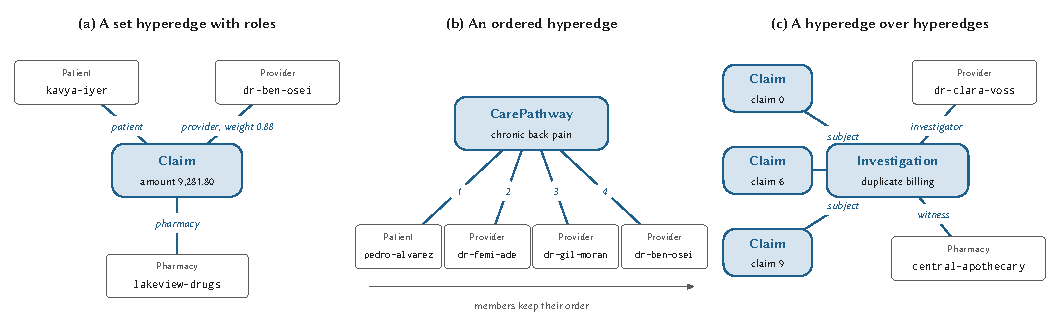
\includegraphics[width=\textwidth]{figures/hypergraph}
\caption{Three hyperedges from the clinical claims example that ships with HStore. (a) A claim relates a patient, a provider and a pharmacy, each in its own role; the provider's membership carries a weight. (b) A care pathway lists a patient and the providers who saw them, in order. (c) An investigation has three claims as its subjects, so its members are themselves hyperedges.}
\label{fig:hypergraph}
\end{figure*}

\Cref{fig:hypergraph} shows one hyperedge of each kind from the example dataset that ships with HStore.

\paragraph{Generations, history and branches.} Every commit produces a new \emph{generation}, numbered consecutively. A reader opens a snapshot of a generation and sees it unchanged for as long as it keeps it open. The engine keeps a configurable number of recent generations (64 by default) for time travel, which can be addressed by number or by wall-clock time. A \emph{branch} is a named line of generations forked from another branch. Creating one copies nothing, and the database layer merges branches with a three-way merge against the fork point.

\paragraph{Operations.} Writes create and delete atoms, change their records, and change memberships: add, update or remove a member by atom, insert, update or remove at a position in an ordered hyperedge, and replace a whole membership in one bulk load. Deleting an atom removes it from every hyperedge that contains it. Reads look up an atom, test and fetch a member, return a hyperedge's cardinality and the member at a given rank, scan members filtered by role, weight or validity time, list the hyperedges incident to an atom, intersect incidence sets (``hyperedges that contain all of $a_1,\dots,a_k$''), and compute differences between two hyperedges, two generations or two branches.

\paragraph{Layers.} The storage engine knows only atoms, memberships and a set of keyed trees. Types, property values, tenants and users, the HQL query language, an embedding index and the higher-order operators are added by a database layer that stores its own data in additional trees inside the same generations (\cref{sec:implementation}). The rest of this paper is about the engine.

\section{Overview}
\label{sec:overview}

\begin{figure*}[t]
\centering
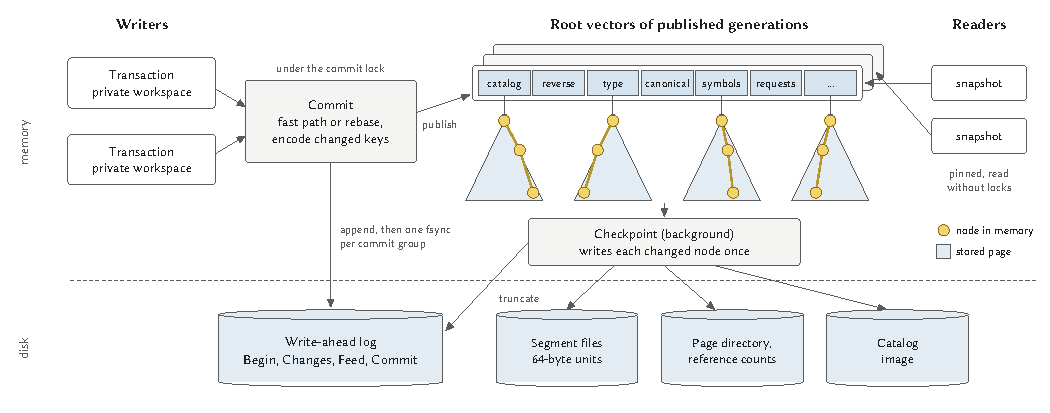
\includegraphics[width=\textwidth]{figures/overview}
\caption{Engine overview. A commit appends the keys it changed to the write-ahead log and publishes a new root vector whose changed nodes (yellow) are still in memory, on top of stored pages (blue). Readers pin a generation and read it without locks. A background checkpoint writes the changed nodes, syncs them, publishes a catalog image and truncates the log.}
\label{fig:overview}
\end{figure*}

\Cref{fig:overview} shows the main parts of the engine. The state of the database at one point in time is a \emph{generation}: a small immutable object that holds, for each branch, a \emph{root vector} that maps a slot number to the root of a tree. The engine defines seven slots: the \emph{catalog} of atoms, the reverse incidence index, an index from type to atoms, an index of canonical keys, two symbol tables for role names, and a table of request ids that makes retried commits idempotent. The database layer adds its own slots for schemas, properties, property indexes and the like. Slots are either primary, written by transactions, or derived, maintained from the primary slots inside the same transaction by \emph{derivations}. The reverse incidence index is derived from the catalog.

All trees are copy-on-write. A transaction works on a private copy of the root vector, and its writes copy the paths they change. A commit publishes a new generation that shares every unchanged subtree with its predecessor. Readers pin a generation and never take a lock. Writers serialise only on a short section of the commit that assigns the generation number and appends to the log, and commits that reach the log while an earlier batch is being synced share one fsync.

The tree nodes a commit creates are not written at commit time. The commit logs the keys it changed and publishes nodes that are still in memory; a background checkpoint later writes them to pages. Pages are packed into append-only segment files and found through a page directory, so that compaction can move them without changing any tree. The rest of the paper follows this structure: trees and the on-disk layout (\cref{sec:layout}), commits, checkpoints and recovery (\cref{sec:transactions}), and reclaiming space (\cref{sec:space}).

\section{Trees and storage layout}
\label{sec:layout}

\subsection{Counted, summarised copy-on-write trees}
\label{sec:tree}

Every tree in HStore is a B+tree over signed 64-bit keys. A leaf holds sorted keys and their values; a branch holds separator keys and child references. Nodes are never changed once another version can see them. An update copies the path from the root to the changed leaf, and the new root shares every other subtree with the old one, as in other copy-on-write B-trees~\cite{lorie,rodeh-shadowing,lmdb}. Inside one transaction, a node that the transaction itself created may be changed in place: each node carries an owner token, and a write copies a node only if its token is not the transaction's. A transaction that makes $n$ changes under one root therefore allocates in proportion to $n$ plus the nodes it touches, not $n$ times the tree height. When a version escapes, for example to a stream handed to the caller, the token is replaced and every node created so far becomes immutable.

Leaves are filled by bytes, not by entry count. A leaf tracks the exact size of its delta-encoded key stream and an upper bound on the size of its values, and splits when the total exceeds the page budget. With the default 16\,KiB page, a leaf of plain 8-byte keys holds thousands of entries and a branch holds up to 137 children.

\paragraph{Summaries.} Each child reference stores the subtree's \emph{summary}, a monoid value made of the entry count, the minimum and maximum key, the sum and range of the entry weights, the range of the validity intervals, a 64-bit mask of the role sets present, and a fingerprint. Combining two summaries is component-wise: sums, minima, maxima and bitwise or. The count makes rank, select and range counts logarithmic, since they subtract or add child counts from the references without loading the children. The other fields let a cursor skip any subtree that cannot hold a match: a scan for members valid at time $t$ enters a child only if $t$ lies in the child's time range, and a scan by role only if the role's bit is set in the mask. The mask is a 64-bucket Bloom filter, so a set bit only means ``maybe'' and the scan checks the role exactly.

\paragraph{Fingerprints.} Let $h(e)$ be a 64-bit hash of an entry. A tree whose order does not matter, such as the members of a set hyperedge, has the fingerprint $F(S)=\sum_{e\in S} h(e) \bmod 2^{64}$, an additive multiset hash~\cite{multiset-hash}. A sequence uses a polynomial hash~\cite{karp-rabin}, $F(e_1\ldots e_n)=\sum_i h(e_i)\,B^{\,n-i} \bmod 2^{64}$, whose concatenation rule $F(LR)=F(L)\,B^{|R|}+F(R)$ lets a branch combine its children's fingerprints. Both depend only on the contents, never on the shape of the tree or the order of insertion. Two hyperedges with different fingerprints differ, and the engine knows it after reading two references. All hashes are computed from explicit mixing functions, not from Java's object hash codes, so fingerprints stay the same across processes and across the native build.

\paragraph{Algebra on shared structure.} Because versions share subtrees, comparing two of them can skip whatever they share. Each reference to a stored subtree is identified by its page number, and two equal references denote the same subtree. A diff walks two frontiers of subtrees and drops a pair of equal references without reading it, so the diff of two consecutive generations costs about twice the tree height in page reads. Counting the intersection of two trees descends both in step: disjoint key ranges contribute nothing, equal references contribute their stored count, and only the parts that differ are read. Intersecting $k$ incidence sets uses a leapfrog join~\cite{leapfrog} over $k$ cursors, each restricted by summaries to the key range common to all inputs. A union of two trees with disjoint key ranges is a concatenation that copies $O(1+\Delta h)$ nodes, where $\Delta h$ is the difference in height.

\subsection{Hyperedges}
\label{sec:hyperedges}

The members of a set hyperedge are a tree keyed by member atom id, whose values are incidences. Membership tests and the member at rank $i$ are logarithmic, and the cardinality is the count in the root reference.

An ordered hyperedge is a sequence that can be edited at any position, so its keys are \emph{order-maintenance labels}~\cite{dietz-sleator,bender-order}: sparse integers in $[0,2^{62})$ whose order is the sequence order. The incidence stores the member id. An insertion between two members takes the midpoint of their labels; an append steps by $2^{24}$, so appending never relabels. When two neighbours have no free label between them, the engine relabels a window around the position, doubling its width until the free space reaches $2^8$ labels per member, which keeps the amortised cost of an insertion logarithmic. A second tree maps each member to its label, so membership tests stay logarithmic. Relabelling changes keys but not contents, so the fingerprint of an ordered hyperedge, which is computed from the incidences and not from their labels, does not change.

Incidence leaves are encoded column by column. A flag byte says which of the six optional columns (roles, weight, start and end of validity, payload, qualifier) any row in the leaf uses. Each such column has a bitmap of the rows that use it, followed by their values as variable-length integers. A plain membership therefore costs one to three bytes, and a leaf whose rows use no optional column is decoded into nothing but an array of member ids.

\begin{figure*}[t]
\centering
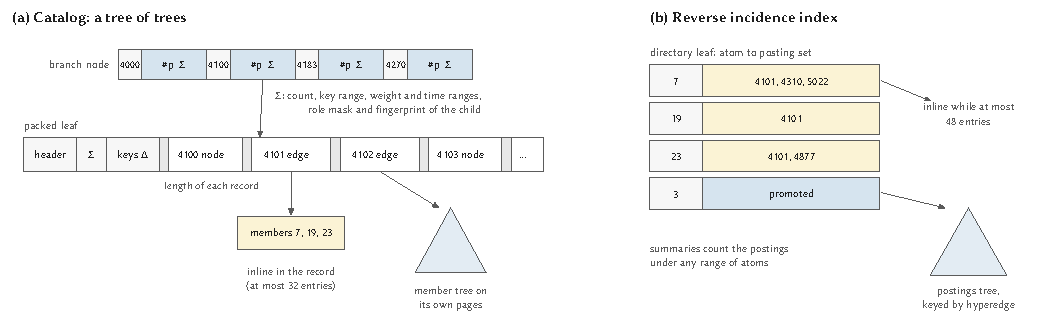
\includegraphics[width=\textwidth]{figures/layout}
\caption{(a) The catalog holds atom records. A hyperedge record holds its membership tree inline when the tree is one small leaf and points to its own pages otherwise. Every record in a catalog leaf is preceded by its length. (b) The reverse incidence index maps an atom to the hyperedges that contain it. Small posting sets are stored in the directory leaf, large ones in a tree of their own.}
\label{fig:layout}
\end{figure*}

\subsection{The catalog: a tree of trees}

The catalog maps an atom id to its record (\cref{fig:layout}a). A hyperedge's record holds references to the root of its membership tree and, for ordered hyperedges, of its label index. These are nested trees that the engine writes, counts and compacts like any other.

Most hyperedges are small: in the dataset of \cref{sec:evaluation}, the mean cardinality is 3.6. Giving each membership a page of its own would cost a page write, a cache entry and a page read for every hyperedge read. A nested tree is therefore kept \emph{inline} in its record when it is a single leaf of at most 32 entries whose encoding fits in 108 bytes, the space a record already reserves for a reference to a tree that is still in memory. That rule keeps pages from overflowing. While a hyperedge is being changed, the leaf that holds its record is sized as if the reference took the full 108 bytes. When the leaf is written, the reference becomes either a stored or an inline one, both of which fit in that space, so the written leaf can only shrink. The decision is made again each time the tree is written, so a hyperedge that grows past the limit moves to its own pages at the next checkpoint and one that shrinks moves back.

\subsection{The reverse incidence index}

The reverse index maps an atom to the hyperedges that contain it (\cref{fig:layout}b). It is a two-level structure. A directory tree maps the atom to a posting set; a posting set maps a hyperedge id to the member's roles and its position key in that hyperedge. A posting set is stored inline in the directory leaf while it has at most 48 entries and at most half the largest value size, and is promoted to a tree of its own beyond that. It is demoted again when it shrinks to 24 entries, so a set that hovers at the limit does not move back and forth. The directory's summaries add up posting counts as weights, so the number of incidences of any range of atoms is read from the summaries alone. The index is a derived slot: a derivation applies every membership change in a transaction to it before the transaction commits, so the two directions always agree within a generation.

\subsection{Node images, page numbers and segments}
\label{sec:pages}

A node is stored as an \emph{image}: an 80-byte header followed by the encoded node. The header holds a magic number, the page type, the tree's schema id, the node's own page number, the generation that wrote it, the payload length, the entry count, the node's summary and a CRC-32C over everything except the checksum itself. Every read verifies the magic number, the format, the page number and the checksum.

A page number is permanent. It has a 48-bit index and 16 bits reserved for reuse, and it says nothing about where the image is stored. The \emph{page directory} maps each index to an address made of a 24-bit segment number, a 24-bit offset in 64-byte units and a 16-bit length in units. The directory is a file of 8-byte entries, memory-mapped in 8\,MiB chunks, so a lookup is one load and takes no Java heap. Trees, the node cache and the log refer only to page numbers; only the page store resolves addresses. Page \code{\#1234}, stored in three units at unit 1234 of segment 1, is the directory entry at byte $64+8\cdot1234$, pointing to byte $64\cdot 1234$ of segment file \code{00000001.seg}.

Images are packed back to back into append-only segment files and aligned to 64 bytes, rather than given a fixed slot of the page size. A hypergraph produces many small nodes, and on the example database that ships with HStore packing cuts the segment space from 17.6\,MB to 1.0\,MB. Each segment is mapped read-only, and a read copies the image out of the map into a heap array before decoding it. Decoding straight from the map was two to five times slower in a microbenchmark, because the JIT compiler generates its fastest code only when every byte buffer that reaches the decoder is of the same kind, and the log and the catalog are decoded from heap arrays.

\subsection{Packed leaves and the node cache}
\label{sec:cache}

Decoded nodes are cached on the Java heap in a node cache with 16 shards. Each shard is an open-addressing table keyed by page number with a CLOCK ring~\cite{clock} for eviction and a byte budget. Lookups are lock-free; only admission takes the shard's lock. A node is charged an estimate of its heap size, computed from its arrays and entries with constants measured against the retained heap at two dataset sizes.

Catalog and index leaves hold variable-length records, and a fully decoded catalog leaf takes far more heap than its page. On our dataset a decoded catalog leaf of about 83 records, with their inline member lists, took about eleven times the size of its 1.5\,KiB image. With a cache smaller than the catalog, lookups missed the cache about half the time and each miss decoded every record of the page to return one. Leaves of codecs whose values are independent of each other therefore prefix every record with its length. A leaf read from a page is kept \emph{packed}: it holds the image, the decoded keys and the offset of every record, and decodes a record the first time it is read. The decoded record is published into the leaf with a compare-and-set, so concurrent readers see a whole record and keep whichever decoding finished first, and its estimated size is charged to the leaf's cache slot. A charge evicts other entries until the shard is back within its budget, and a charge for a slot that was evicted in the meantime is dropped. The length prefix costs about one byte per record; \cref{sec:eval-ablation} measures what it buys.

\section{Transactions and durability}
\label{sec:transactions}

\subsection{Snapshots and isolation}

The transaction manager keeps two generations: \emph{head}, the newest generation appended to the log, and \emph{current}, the newest one that is durable and published. New readers and transactions pin \emph{current}, so no one sees a commit that a crash could still lose. Pins are reference counts per generation. Old generations are trimmed to the history limit, except that a pinned generation is skipped rather than treated as a barrier, so one long-running reader keeps only its own generation alive. Reading an old generation costs the same as reading the newest one: copy-on-write never changes a page that a retained generation can reach, so time travel needs no undo log.

Transactions run under snapshot isolation by default~\cite{critique}. Under the serializable level, a transaction records the value of every key and atom it reads as of its base generation, and a commit that has to rebase (below) checks that none of them changed. This rejects write skew, at key granularity and only when a slot the transaction read has moved.

\subsection{Commit}

A transaction keeps an \emph{operation log}: every operation it applied, stored as an intent such as ``insert member $m$ into hyperedge $e$'' or ``update key $k$ of slot $s$ if its value is still $v$''. The operations are also applied immediately to the transaction's private copy of the trees, and the derivations update the derived slots in the same copy.

At commit, the transaction takes the commit lock and compares its base root vector with \emph{head}. If no slot it changed has moved, it takes the fast path: the new root vector is \emph{head}'s with the transaction's changed slots laid over it. Commits that write different slots therefore never wait for each other, however many commits land in between. Otherwise the commit replays its operation log against \emph{head}. Replay fails with a retryable conflict when a precondition no longer holds, with one exception that matters for hypergraphs. When the only change to a set hyperedge was other transactions adding or removing members, and every action of this transaction on it named a member, the commit diffs the hyperedge's old and new membership trees and conflicts only if a changed member is one it touched. Two transactions that add different members to the same hyperedge therefore both commit. Positional actions on ordered hyperedges and bulk loads conflict whenever the hyperedge moved. A commit can carry a request id. It is recorded in a slot under the commit lock, so a retried commit returns the original generation instead of applying twice.

\subsection{Logging keys instead of pages}

A copy-on-write commit that writes its new pages writes every node from each changed leaf up to the root of each changed tree. For one updated property, that is a few leaves and branches in the property tree, its index and the catalog, many kilobytes for a few bytes of change. HStore commits instead log the keys they changed and publish a generation whose new nodes are still in memory.

The write-ahead log is a sequence of segment files addressed by a log sequence number (LSN), the byte offset since the log was created. Every record is a frame with a 25-byte header that holds the payload length, a CRC-32C, the frame's own LSN, the record type and the transaction id. Because the checksum covers the LSN, stale bytes left in a reused file can never pass for a valid frame. A commit appends, under the commit lock, a \code{Begin} record, one \code{Changes} record, a \code{Feed} record with the commit's logical events for the change feed, and then, in a separate append, the \code{Commit} record with the generation number and the next free atom and transaction ids. The \code{Commit} frame is the commit point.

The \code{Changes} payload lists, for each slot whose root changed, the keys that differ between the base tree and the new one, found with the diff of \cref{sec:tree}. A changed value that holds nested trees, such as a hyperedge record, is followed by the changes to each nested tree, so a commit that adds one member to a hyperedge logs that member, not the hyperedge. A tree that changed in more than 4,096 places, as after a large bulk load, is written to pages at commit and logged by reference instead. Each such page gets a 47-byte \code{PageRef} record with its page number, address, length and CRC-32C, and the data files are forced before the log whenever a commit group contains such pages. Large bulk loads also \emph{spill} finished subtrees to pages while they run, so that a hyperedge with millions of members never has to fit in memory.

Commits do not wait for the disk under the commit lock. The lock is released after the \code{Commit} frame is appended, and the committing thread then waits on a group committer. The group committer has no thread of its own: the first waiting committer becomes the leader, takes every queued commit as one batch, syncs once, publishes the batch in generation order and wakes the others. Under synchronous durability the batch forces the data files if any of its commits wrote pages and then the log; under asynchronous durability nothing is forced, but publication order is the same. Commits that arrive while a batch is syncing form the next batch, so the batch size grows with the number of concurrent writers.

\subsection{Checkpoints}

A checkpoint writes the trees of one published generation $g$ to pages and makes it the starting point of the next recovery. It walks the roots of $g$ and writes every node that is still only in memory, children before parents. Each written node is stamped with its stored reference and the checkpoint's \emph{epoch}; when the epoch is published, the next checkpoint reuses these pages and does not visit the subtrees below them. A node that many commits changed between two checkpoints is written once. The checkpoint then forces the data files and the page directory, updates the page reference counts (\cref{sec:space}), journals them, and publishes a catalog image that records $g$'s roots, the segment table and the checkpoint LSN, the end of $g$'s \code{Commit} frame. The image is written to a temporary file, forced, renamed and the directory forced. Last, the log is truncated before the checkpoint LSN.

Commits continue during all of this. The log is forced outside the lock that appends to it, so a commit appending its records never waits for the checkpoint's sync. By the time the checkpoint publishes, \emph{head} may be several generations past $g$ and still refer to the in-memory nodes that the checkpoint wrote. The checkpoint swaps every node it wrote in \emph{head} for its stored reference, copying only the parents whose children changed. It does this in two passes. The first runs without any lock and remembers its result for every node it visits. The second runs under the commit lock over the newest \emph{head}, reuses those results and only walks what commits added in between, so the commit lock is held for the part of the tree that changed during the first pass. A transaction that started before the checkpoint still compares equal: an in-memory node stamped by a published epoch is treated as the same tree as the reference it was written as, so a finished checkpoint never pushes a transaction off the fast path.

The heap held by unwritten nodes is capped (64\,MiB by default), and a checkpoint starts when half of the cap is used. It also starts when the log or the pages written since the last checkpoint pass a threshold, or when more than a million reference counts have changed. By default the threshold is a quarter of the live bytes in the data segments, but at least 2\,MiB and at most 256\,MiB, so that the log a crash leaves to replay stays small relative to the store while a large store does not checkpoint more often than a fixed 256\,MiB would. A database can fix the threshold with the statement \code{CHECKPOINT AT 64MB}, which is stored in the database, and \code{CHECKPOINT AT AUTO} returns to the default. A background thread checks these conditions every 500\,ms, and a commit that pushes the log past the threshold wakes it at once. A commit that finds the cap reached waits for a checkpoint to make room.

\begin{figure*}[t]
\centering
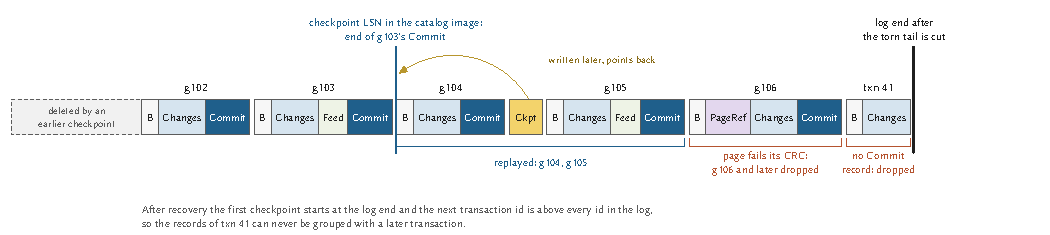
\includegraphics[width=\textwidth]{figures/wal}
\caption{Recovery reads the log from the checkpoint LSN recorded in the newest catalog image. It replays every commit whose \code{Commit} frame is valid, stops at the first commit whose referenced pages do not verify, and drops the records of transactions that never committed.}
\label{fig:wal}
\end{figure*}

\subsection{Recovery}
\label{sec:recovery}

Opening a database (\cref{fig:wal}) loads the newest valid catalog image, cuts the log's last segment at the end of its last valid frame, and reads the log from the image's checkpoint LSN. Records are grouped by transaction id. For each \code{Commit} frame in log order whose generation is newer than the image, recovery first restores the directory entries of the pages the commit references, then checks that every page referenced by a \code{PageRef} reads back with a valid header and the logged checksum, and then applies the commit's \code{Changes} to the trees of the previous generation. The replayed generations live in memory, exactly as they did before the crash, and the checkpoint that ends every open writes them.

Two rules make the recovered state a prefix of the commit order. First, a commit is part of the recovered state only if its \code{Commit} frame is in the log; records of transactions that never committed are dropped. Second, if one commit's pages fail verification, it and every later commit are dropped. The second rule matters after a power failure: the operating system may write the log to disk before the data pages it refers to, and a later commit's key changes apply to the trees of the commit before it, so replaying it on top of a lost commit would produce a state that never existed. Only commits that wrote pages can hit this rule, and none of them had been acknowledged, because acknowledgement comes after both syncs.

Recovery also guards against reusing what the log still holds. Transaction ids are persisted only in \code{Commit} records, so the id of a transaction that died during its commit would otherwise be handed out again while its records were still in the log, and a second crash would let recovery group the dead records with the new transaction's. Recovery therefore sets the next transaction id above every id it saw in the log, and the checkpoint at the end of the open starts from the end of the log rather than from the old checkpoint LSN, so those records are never read again.

Recovery writes nothing to the log, and the only state it leaves behind is published by the checkpoint at the end of the open, so a crash during recovery repeats the same work on the next open. History is not part of the catalog image. After a restart, time travel reaches the checkpointed generation and the generations replayed after it, and older states are available only through the change feed.

\section{Reclaiming space}
\label{sec:space}

Copy-on-write never overwrites a page, so every checkpoint leaves behind the images it replaced. They stay reachable while a retained generation refers to them and become garbage afterwards. Segments are append-only, so garbage is never reused piece by piece: HStore copies the live images out of mostly dead segments and deletes the files. This needs two things, knowing which images are live and moving them without touching the trees that point at them.

\subsection{Reference counts between checkpoints}

Every page number has a reference count in a memory-mapped file laid out like the directory. The count is the number of places that point at the page in the last checkpointed generation: a slot root, a child reference in a branch, or a nested tree's root inside a record. Inline trees have no page and are never counted. A negative entry marks a page that died in generation $d$ and is waiting until no reader can see a generation older than $d$.

Counts change only at checkpoints, and only between two generations whose trees are fully written: the one the previous checkpoint wrote and the one the current checkpoint just wrote. Generations published in between are never counted. Their new nodes have no pages, and every page they reach was counted by the previous checkpoint or is \emph{provisional} (spilled by a bulk load or written by a large commit, and resolved by the checkpoint that covers it). For each branch whose roots changed, the counter first adds one to every new root, recursing into a page only when its count rises from zero, and then subtracts one from every old root, recursing only when a count reaches zero. When a node is replaced, its children are added by the new copy and subtracted by the old one, so they cancel and are never touched. The work is proportional to the pages that changed between the two checkpoints, not to the number of commits or the size of the trees. Most of the nodes it reads are in the node cache because the checkpoint has just written them. A header flag records whether a leaf refers to any page, so leaves that hold only plain records or inline trees, such as most catalog leaves, are never decoded.

A page that died in generation $d$ is released at a checkpoint once $d$ is no newer than the oldest generation anyone can still read, the older of the oldest retained and the oldest pinned generation. Releasing clears its directory entry and subtracts its bytes from its segment's live total. The changed counts and the cleared entries are journaled with absolute values before the catalog image is published and applied afterwards, so a crash leaves the files as of one checkpoint or the next, never a mix, and applying a journal twice is harmless.

\begin{figure}[t]
\centering
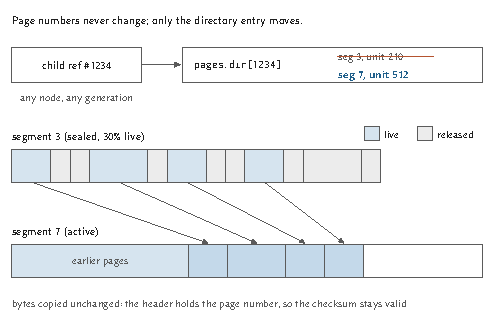
\includegraphics[width=\columnwidth]{figures/compaction}
\caption{Compaction copies the live images of a mostly dead segment to the active segment and changes their directory entries. Every tree, in every generation and branch, still refers to the same page numbers.}
\label{fig:compaction}
\end{figure}

\subsection{Compaction by moving}

A sealed segment whose live bytes fall below a threshold (half of the bytes written to it, by default) is a compaction victim. Compaction reads through the victim one 64-byte unit at a time (\cref{fig:compaction}). Where a header starts and the directory entry for that header's page number points at exactly this place, the image is live: it is verified and its bytes are appended to the active segment. Anything else, such as a released image or an older copy of a moved one, is skipped. The header holds the page number, not the address, so neither the header nor the checksum changes. After every 4\,MiB of copies the segments are forced, and only then are the directory entries pointed at the copies, so an entry never reaches the disk ahead of the bytes it points to. The victim is then retired, and its file is deleted after the next checkpoint has made the new entries durable and once no pinned reader started before the move.

Nothing in this takes the commit lock or commits anything. Commits continue while pages move, cached nodes stay valid because they are keyed by page number, and old generations reach the moved pages through the same directory, so compaction never shortens the time-travel window. Moves are not logged. If the engine crashes before the checkpoint that follows a compaction, recovery restores the directory entries of the replayed commits to their original addresses, which are still intact because victims are deleted only after that checkpoint. The copies become unreferenced space that a later pass reclaims. The work is proportional to the size of the victims, and the only memory it needs is the list of pages moved in the current 4\,MiB.

A background pass compacts the emptiest victim every 500\,ms if one exists; an explicit request compacts all of them. A new segment gets 8\,MiB, doubled as long as it stays within an eighth of the bytes in the other segments, up to 256\,MiB. A small database therefore has several sealed segments for compaction to choose from, and a large one has few files. The engine keeps at most 256 segment files open and closes the least recently used one, after forcing it if it has unsynced writes, so the number of open files does not grow with the database.

\section{Implementation}
\label{sec:implementation}

HStore is written in Java~25 as three modules. The storage engine (about 12,000 non-blank lines) depends only on the Java base module. The database layer (about 7,900 lines) adds schemas and typed properties, property indexes, tenants and users, evidence and valid-time queries, a three-way branch merge, an embedding index fed from the change feed, higher-order operators over incidence sets, and HQL, a query language with a cost-based planner. The server (about 2,600 lines) provides a command-line tool, a line-oriented TCP protocol and a web console. The same code runs on the JVM and as a GraalVM native image, which is how the server ships in its container image.

The engine leans on recent additions to the Java platform. Segment maps and the page directory use the foreign memory API; each segment map has its own shared arena and is closed as soon as the segment is remapped or deleted, so the disk space of a deleted segment comes back at once instead of when the garbage collector finds the mapping. A per-query I/O meter, which enforces a page budget per query, is bound with scoped values rather than thread-locals. Server connections and feed subscribers run on virtual threads. Commits can therefore be issued from thousands of threads, and the group committer runs its sync on whichever committing thread leads the batch.

A Java thread that is interrupted during a read or write on a \code{FileChannel} closes the channel for every thread. Before this was handled, one request that timed out during a commit closed the log and every later commit failed. All shared files are therefore accessed through a wrapper that clears the interrupt flag for the length of the call, restores it afterwards, and reopens the file and retries if the channel was closed anyway; every read and write is positional, so a retry touches the same bytes.

\paragraph{Testing.} The engine's tests inject a crash at each of fourteen named points: the seven steps of a commit from the first page write to publication, two steps of compaction, four of a checkpoint and the force of the log. Each commit crash point is run with both log modes; the test asserts that the reopened store holds either the state before the commit or the state after it, never a mix, and that the forward and reverse indexes agree. A second set of tests models a power failure instead of a process crash. Every file the engine writes is opened through one wrapper, which lets a test record each write, each sync of a file or a memory map and each sync of a directory, cut the power at any of these events, and rebuild the directory as a disk could have kept it: only what was synced, the last unsynced write torn in half or with a flipped byte, or a random mix, with files whose directory was never synced possibly missing. The tests then check that the recovered commits are a prefix of the attempted ones, that every commit acknowledged under synchronous durability survived, that no aborted work appears and that the change feed holds exactly one event per recovered commit. They found five bugs, all of them in files outside the log: a format marker written without a sync, a segment directory that was never synced after a file was created in it, a page directory header that could keep an unsynced first page number, and two ways in which zeroed or damaged change-feed frames were read as valid. After random workloads, the suites replay the log against the generations in memory and compare them entry by entry, and a verifier checks every reachable page (checksums, key order, balance, summaries and reference counts), which the \code{hstore check} command also runs. Finally, we kill the native server with SIGKILL during a bulk load, reopen it and check the counts.

\section{Evaluation}
\label{sec:evaluation}

We compare HStore with HyperGraphDB, the only other embedded store we know of whose atoms are hyperedges with a variable number of members. The evaluation asks four questions. How do the two systems compare on reads, writes and space when the data fits in the cache and when it does not (\cref{sec:eval-throughput,sec:eval-resources})? What do commits and reads cost one at a time, and how do reads behave while a writer is committing (\cref{sec:eval-latency})? How do the systems recover from a crash and reclaim space after deletes (\cref{sec:eval-space})? And how much does each of HStore's main design decisions contribute (\cref{sec:eval-ablation})?

\subsection{Setup}
\label{sec:eval-setup}

\paragraph{Dataset.} The dataset is generated from a fixed seed, so both systems load the same hypergraph. At scale $s$ it has $50{,}000\,s$ nodes and $100{,}000\,s$ hyperedges. A hyperedge starts with two members and gains each further member with probability 0.62, up to 32, for a mean cardinality of 3.6. Members are drawn as $\lfloor n u^{2.2}\rfloor$ for uniform $u\in[0,1)$ over $n$ nodes, so low-numbered nodes become hubs. At scale~1 half of the nodes are in at most 5 hyperedges, 370 are in more than 48, and the largest is in 2,645; at scale~4 the largest is in 5,714. Probe sets from the same seed select 100,000 random atoms, 20,000 pairs of nodes that share a hyperedge, and 20,000 node updates. A churn set selects 20\% of the hyperedges for deletion and 20,000 other hyperedges, each losing one member.

\paragraph{Workloads.} \Cref{tab:workloads} lists the \M{workloadCount} workloads, which run in this order in one process per system and run. Each adapter uses the plain storage API of its system: long ids and \code{forEachIncidentEdge}, \code{forEachMemberId} and \code{Writer.set} for HStore, persistent handles and \code{getIncidenceSet}, \code{getTargetAt} and \code{graph.replace} for HyperGraphDB. We do not use HyperGraphDB's traversal framework, so that both sides measure storage. HyperGraphDB links are immutable, so removing a member replaces the link. Every read and delete workload returns a checksum, such as the number of ids visited, and both systems returned the same checksum in every run.

\begin{table}[t]
\centering\footnotesize
\caption{Workloads, in execution order.}
\label{tab:workloads}
\begin{tabularx}{\columnwidth}{@{}lX@{}}
\toprule
Workload & Operation \\
\midrule
\wl{ingest.nodes}, \wl{.edges} & insert all nodes, then all hyperedges, 1,000 per transaction \\
\wl{read.incidence} & list the hyperedges that contain a node; 100,000 probes \\
\wl{read.members} & list a hyperedge's members; 100,000 probes \\
\wl{read.comembership} & count the hyperedges that contain both nodes of a pair \\
\wl{read.twohop} & count distinct nodes that share a hyperedge with a node \\
\wl{read.incidence.parallel} & \wl{read.incidence} from 8 threads \\
\wl{latency.read} & one incidence lookup per read transaction, each timed \\
\wl{write.update} & replace a node's value; 20,000 updates, 1,000 per transaction \\
\wl{latency.commit} & one update per transaction, each timed; 5,000 commits \\
\wl{mixed.read}, \wl{.write} & 7 reader threads for 10\,s beside a writer committing 10 updates per transaction on a fixed schedule of 1,000 updates/s \\
\wl{large.*} & create one hyperedge that contains every node, scan it 400 times, probe it 100,000 times \\
\wl{reopen} & close cleanly and open again \\
\wl{read.incidence.cold} & \wl{read.incidence} right after the reopen \\
\wl{churn.delete}, \wl{.remove} & delete 20\% of the hyperedges; remove one member from 20,000 others \\
\wl{compaction} & single-update commits at 50/s while a full space reclamation runs \\
\wl{disk}, \wl{.churned}, \wl{.compacted} & bytes on disk after load, after the deletes, after reclamation \\
\wl{recover} & open a store whose ingest process was killed with SIGKILL \\
\bottomrule
\end{tabularx}
\end{table}

\paragraph{Measurement.} Throughput is the operation count divided by the elapsed time of the whole operation set. Each write workload ends with a flush outside the timed section (an HStore checkpoint or a JE \code{sync}), so bytes still in buffers are charged to the workload that produced them. Every read workload except \wl{read.incidence.cold} first runs untimed for at least 2\,s, so both systems are measured with their read paths compiled by the JIT. The latency workloads time every transaction; in \wl{mixed} and \wl{compaction} the writer follows a fixed schedule and its latency is measured from the scheduled start, so a stall is charged to every commit queued behind it~\cite{fair-benchmarking}. Both systems count their own file I/O: HStore its log and page bytes, including pages moved by compaction, and HyperGraphDB the bytes JE writes and reads, including its cleaner. Allocation per operation comes from the JVM's per-thread allocation counters and the retained heap from a full collection after ingest.

\paragraph{Configurations.} We run three configurations. S1~async is scale~1 with asynchronous commits. S1~sync is scale~1 with synchronous commits. S4~async is scale~4 with asynchronous commits; there the files of both systems are larger than their 64\,MiB caches. Both caches get the same 64\,MiB budget. HStore's covers decoded nodes; JE's covers its B+tree nodes and records, and HyperGraphDB's atom cache comes on top and cannot be capped in bytes. HyperGraphDB~1.4 begins every JE transaction with \code{WRITE\_NO\_SYNC}, which overrides the environment's \code{COMMIT\_SYNC}; under S1~sync its adapter therefore forces JE's log after every commit, which is what \code{COMMIT\_SYNC} would do.

\paragraph{Machine.} All runs used one Azure \code{Standard\_D8ds\_v5} virtual machine: four cores (eight hardware threads) of an Intel Xeon Platinum 8370C at 2.8\,GHz, 32\,GiB of memory, and Ubuntu 24.04 with Linux 6.17. Both systems kept their files on the machine's local 300\,GB temporary SSD, formatted as ext4, and ran on Oracle GraalVM 25.0.4 in JVM mode. HyperGraphDB is version 1.4 built from commit \code{99485a1} with Berkeley DB JE 5.0.73, the JE version its storage module is written against. Each system runs in its own JVM with a fixed 4\,GiB heap and the Parallel collector. Runs alternate between the two systems, so that a slow period on the machine affects both. We report medians over \M{runss1async}, \M{runss1sync} and \M{runss4async} runs per system for the three configurations. A ratio is oriented so that values above 1 favour HStore, and it is marked with $\dagger$ when the ranges of the two systems' runs overlap.

\begin{table*}[t]
\centering\footnotesize
\caption{Median results. Rates are operations per second; \wl{disk} rows are bytes on disk; \wl{reopen} and \wl{recover} are times. A ratio above 1 favours HStore, and $\dagger$ marks a ratio whose run ranges overlap. The S1~sync column gives only the ratio; its rates differ from S1~async only for the commit-bound workloads discussed in the text.}
\label{tab:results}
\begin{tabular}{@{}lrrrrrrr@{}}
\toprule
& \multicolumn{3}{c}{S1 async} & S1 sync & \multicolumn{3}{c}{S4 async} \\
\cmidrule(lr){2-4}\cmidrule(lr){5-5}\cmidrule(l){6-8}
Workload & HStore & HyperGraphDB & ratio & ratio & HStore & HyperGraphDB & ratio \\
\midrule
\wl{ingest.nodes} & 33.3\,k & 19.6\,k & 1.7 & 1.7 & 42.9\,k & 24.0\,k & 1.8 \\
\wl{ingest.edges} & 28.9\,k & 21.3\,k & 1.4 & 1.3 & 21.5\,k & 2.71\,k & 7.9 \\
\wl{read.incidence} & 3.10\,M & 1.25\,M & 2.5 & 3.1 & 2.62\,M & 1.11\,M & 2.4 \\
\wl{read.members} & 2.29\,M & 1.66\,M & 1.4 & 1.6 & 2.13\,M & 1.27\,M & 1.7 \\
\wl{read.comembership} & 272\,k & 49.8\,k & 5.5 & 4.9 & 281\,k & 41.4\,k & 6.8 \\
\wl{read.twohop} & 243\,k & 83.6\,k & 2.9 & 3.4 & 172\,k & 80.9\,k & 2.1 \\
\wl{read.incidence.parallel} & 14.1\,M & 1.28\,M & 11 & 12.8 & 8.21\,M & 1.26\,M & 6.5 \\
\wl{latency.read} & 2.07\,M & 505\,k & 4.1 & 3.8 & 1.79\,M & 470\,k & 3.8 \\
\wl{write.update} & 40.9\,k & 7.26\,k & 5.6 & 5.8 & 30.2\,k & 2.47\,k & 12.2 \\
\wl{latency.commit} & 6.96\,k & 7.33\,k & 0.95$^\dagger$ & 1.2 & 10.1\,k & 2.54\,k & 4.0 \\
\wl{mixed.read} & 8.73\,M & 1.13\,M & 7.7 & 8.0 & 8.55\,M & 1.11\,M & 7.7 \\
\wl{mixed.write} & 1,000 & 1,000 & 1.0 & 1.0 & 1,000 & 999 & 1.0 \\
\wl{large.ingest} & 431\,k & 47.6\,k & 9.1 & 7.4 & 489\,k & 13.6\,k & 36.1 \\
\wl{large.scan} & 1,668\,M & 344\,M & 4.8 & 4.5 & 1,583\,M & 358\,M & 4.4 \\
\wl{large.probe} & 6.60\,M & 1.01\,M & 6.5 & 7.2 & 5.61\,M & 844\,k & 6.7 \\
\wl{reopen} & 78.5\,ms & 978\,ms & 12.5 & 13 & 92.9\,ms & 1,279\,ms & 13.8 \\
\wl{read.incidence.cold} & 1.73\,M & 67.6\,k & 25.6 & 28.1 & 1.23\,M & 15.1\,k & 81.6 \\
\wl{disk} & 85.7\,MiB & 400\,MiB & 4.7 & 4.3 & 172\,MiB & 2.30\,GiB & 13.7 \\
\wl{churn.delete} & 16.1\,k & 5.18\,k & 3.1 & 2.9 & 2.64\,k & 1.99\,k & 1.3 \\
\wl{churn.remove} & 23.1\,k & 10.7\,k & 2.2 & 2.1 & 4.08\,k & 3.53\,k & 1.2 \\
\wl{read.incidence.churned} & 3.10\,M & 1.30\,M & 2.4 & 2.6 & 2.75\,M & 1.05\,M & 2.6 \\
\wl{disk.churned} & 116\,MiB & 293\,MiB & 2.5 & 2.0 & 1.14\,GiB & 1.91\,GiB & 1.7 \\
\wl{compaction.baseline} & 50.1 & 50.1 & 1.0$^\dagger$ & 1.0$^\dagger$ & 50.1 & 50.1 & 1.0 \\
\wl{compaction} & 50.1 & 50.1 & 1.0$^\dagger$ & 1.0$^\dagger$ & 50.1 & 50.0 & 1.0 \\
\wl{disk.compacted} & 93.3\,MiB & 234\,MiB & 2.5 & 2.7 & 183\,MiB & 1.15\,GiB & 6.4 \\
\wl{recover} & 84.8\,ms & 113\,ms & 1.3$^\dagger$ & 1.4 & 162\,ms & 449\,ms & 2.8 \\
\bottomrule

\end{tabular}
\end{table*}

\begin{figure}[t]
\centering
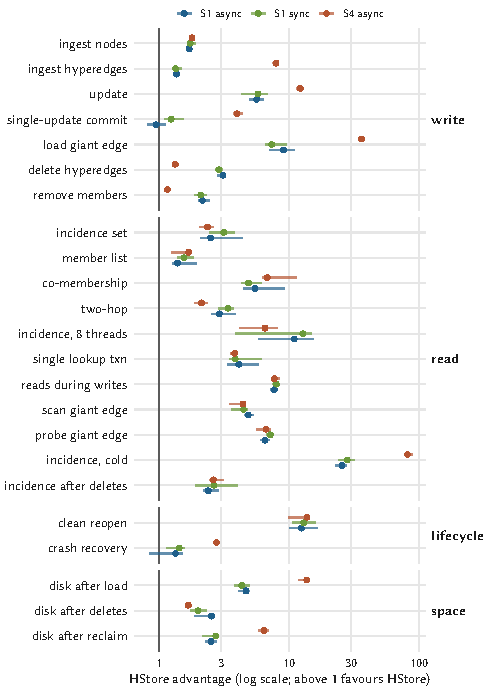
\includegraphics[width=\columnwidth]{figures/ratios}
\caption{HStore's advantage per workload and configuration: the ratio of the medians, with a bar from the least to the most favourable pairing of runs. Workloads with a fixed rate are left out.}
\label{fig:ratios}
\end{figure}

\subsection{Throughput}
\label{sec:eval-throughput}

\Cref{tab:results} lists every median and \cref{fig:ratios} plots the ratios. Every read and delete workload returned the same checksum on both systems in every run. HStore is ahead on every workload whose rate the harness does not fix, with one exception: single-update commits under asynchronous durability at scale~1, where the two systems are within each other's range (\M{ratios1asynclatencycommit}).

\paragraph{Reads.} A batch of incidence lookups is \M{ratios1asyncreadincidence} times faster at scale~1 and \M{ratios4asyncreadincidence} times faster at scale~4, and member lookups are \M{ratios1asyncreadmembers} and \M{ratios4asyncreadmembers} times faster. Counting the hyperedges two nodes share is \M{ratios1asyncreadcomembership} times faster at scale~1. HStore answers it by intersecting the two incidence trees and skipping every pair of subtrees whose key ranges do not overlap; HyperGraphDB evaluates the conjunction of two incidence conditions. From eight threads HStore reaches \M{hss1asyncreadincidenceparallel} incidence lookups per second at scale~1, while HyperGraphDB stays at \M{hgs1asyncreadincidenceparallel}, about its single-thread rate of \M{hgs1asyncreadincidence}. Right after a reopen the gap is widest: \M{ratios1asyncreadincidencecold} times at scale~1 and \M{ratios4asyncreadincidencecold} times at scale~4. HStore reads its segments through memory maps that the operating system's page cache still holds and decodes a leaf record only when it is read, while JE fills its own cache from its log one node at a time.

\paragraph{Writes.} Node and hyperedge ingest are \M{ratios1asyncingestnodes} and \M{ratios1asyncingestedges} times faster at scale~1. At scale~4, where both systems' files outgrow their 64\,MiB caches, hyperedge ingest is \M{ratios4asyncingestedges} times faster, because HyperGraphDB drops from \M{hgs1asyncingestedges} to \M{hgs4asyncingestedges} hyperedges per second. Updates in batches of 1,000 are \M{ratios1asyncwriteupdate} and \M{ratios4asyncwriteupdate} times faster. Creating one hyperedge that holds every node is \M{ratios1asynclargeingest} times faster at scale~1 and \M{ratios4asynclargeingest} times at scale~4, and scanning it is \M{ratios1asynclargescan} times faster. Deletes are the closest. At scale~4 HStore deletes \M{hss4asyncchurndelete} hyperedges per second, \M{ratios4asyncchurndelete} times HyperGraphDB's rate, against \M{ratios1asyncchurndelete} times at scale~1. Deleting a hyperedge removes it from the reverse index of every member, and at scale~4 those postings are spread over many more pages than the cache holds.

\paragraph{Opening a database.} A clean reopen takes \M{hss1asyncreopen} against \M{hgs1asyncreopen} at scale~1 (\M{ratios1asyncreopen} times faster). HStore loads the catalog image and maps the segments; nothing is replayed after a clean shutdown.

\subsection{Latency}
\label{sec:eval-latency}

\begin{figure*}[t]
\centering
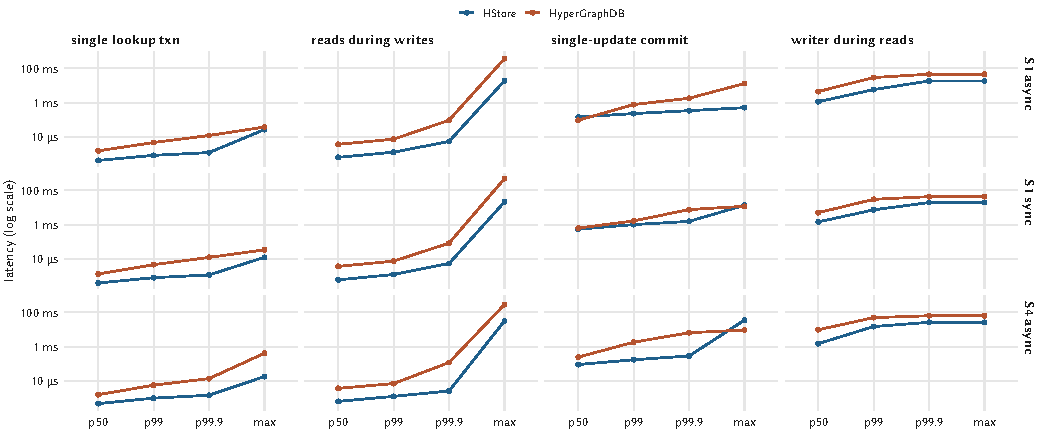
\includegraphics[width=\textwidth]{figures/latency}
\caption{Latency percentiles, medians over runs. Read latencies are per transaction with one lookup; commit latencies include the wait for the group commit; in the mixed workload the writer's latency is measured from each transaction's scheduled start.}
\label{fig:latency}
\end{figure*}

\Cref{fig:latency} shows the percentiles. A read transaction that looks up one incidence set takes \M{lats1asynclatencyreadhspfifty} at the median on HStore and \M{lats1asynclatencyreadhgpfifty} on HyperGraphDB, and \M{lats1asynclatencyreadhspninetyninenine} against \M{lats1asynclatencyreadhgpninetyninenine} at the 99.9th percentile.

Single-update commits are where the systems are closest. Under asynchronous durability at scale~1, HyperGraphDB's median commit is faster (\M{lats1asynclatencycommithgpfifty} against \M{lats1asynclatencycommithspfifty}), but its tail is longer: \M{lats1asynclatencycommithgpninetynine} against \M{lats1asynclatencycommithspninetynine} at the 99th percentile and \M{lats1asynclatencycommithgpninetyninenine} against \M{lats1asynclatencycommithspninetyninenine} at the 99.9th. Under synchronous durability every commit waits for an fsync, and HStore's median is \M{lats1synclatencycommithspfifty} against \M{lats1synclatencycommithgpfifty}; a commit writes \M{writtens1synclatencycommiths} to HStore's log and data files and \M{writtens1synclatencycommithg} to JE's. At scale~4 HStore's commits are faster at every percentile up to the 99.9th (\M{lats4asynclatencycommithspninetyninenine} against \M{lats4asynclatencycommithgpninetyninenine}), but its slowest commit in a run is slower: \M{lats4asynclatencycommithsmax} at the median of the runs against \M{lats4asynclatencycommithgmax}. We have not yet traced these single stalls.

The mixed workload runs seven readers for 10\,s beside a writer that commits 1,000 updates per second on a fixed schedule. Both writers kept the schedule. HStore's readers complete \M{ratios1asyncmixedread} times as many lookups, with a median latency of \M{lats1asyncmixedreadhspfifty} against \M{lats1asyncmixedreadhgpfifty} and a 99.9th percentile of \M{lats1asyncmixedreadhspninetyninenine} against \M{lats1asyncmixedreadhgpninetyninenine}. HStore readers never take a lock, so the writer does not slow them, and the writer in turn finishes its transactions sooner: its 99th percentile, measured from the scheduled start, is \M{lats1asyncmixedwritehspninetynine} against \M{lats1asyncmixedwritehgpninetynine}.

\subsection{Resources}
\label{sec:eval-resources}

\begin{figure*}[t]
\centering
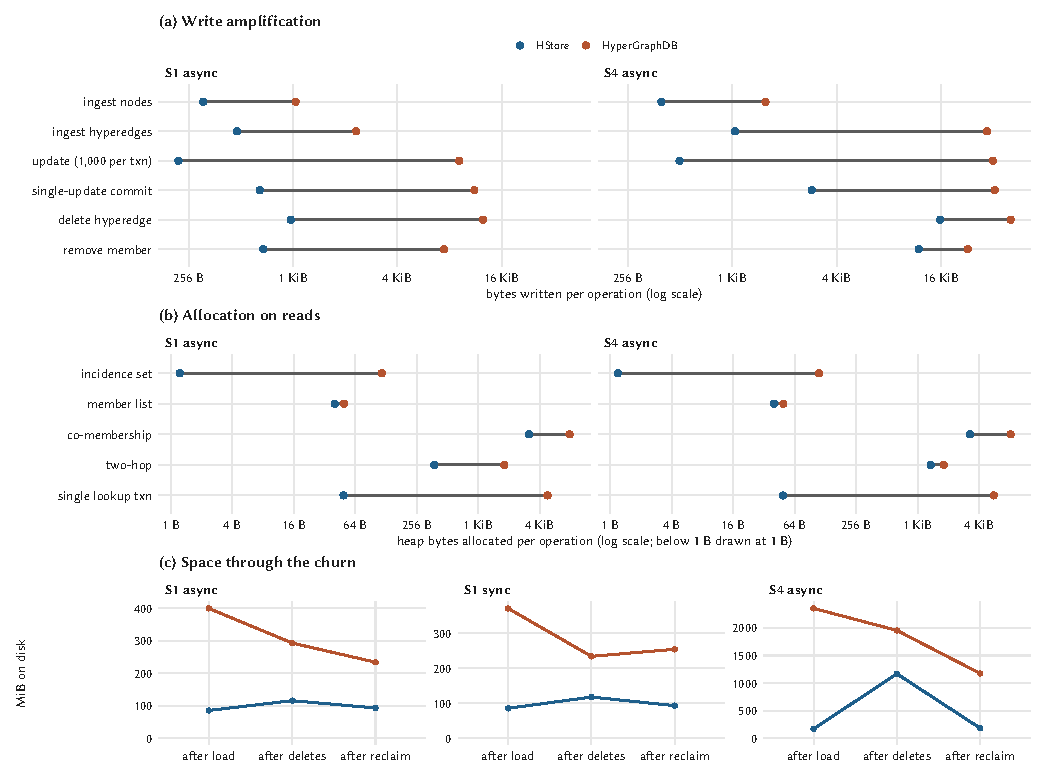
\includegraphics[width=\textwidth]{figures/resources}
\caption{(a) Bytes written to the log and data files per operation, including JE's cleaner and HStore's compaction. (b) Heap bytes allocated per operation on the read workloads, over all threads. (c) Bytes on disk after the load, after the deletes and after reclamation, each measured after a clean shutdown.}
\label{fig:resources}
\end{figure*}

\paragraph{Bytes written.} Logging keys instead of pages shows most clearly in the bytes written per change (\cref{fig:resources}a). An update in a batch writes \M{writtens1asyncwriteupdatehs} on HStore and \M{writtens1asyncwriteupdatehg} on HyperGraphDB, and a single-update commit \M{writtens1asynclatencycommiths} against \M{writtens1asynclatencycommithg}. At scale~4 hyperedge ingest writes \M{writtens4asyncingestedgeshs} per hyperedge against \M{writtens4asyncingestedgeshg}. Over a whole run at scale~4, HStore wrote \M{totalwrittens4asynchs} and HyperGraphDB \M{totalwrittens4asynchg}, \M{compactwrittens4asynchg} of it during the \wl{compaction} workload, while JE's cleaner copied live records out of old log files after the deletes.

\paragraph{Allocation and heap.} Reads on HStore allocate almost nothing (\cref{fig:resources}b): \M{allocs1asyncreadincidencehs} per incidence lookup in a batch against \M{allocs1asyncreadincidencehg}, and \M{allocs1asynclatencyreadhs} per single-lookup transaction against \M{allocs1asynclatencyreadhg}. In the mixed workload, where the readers allocate \M{allocs1asyncmixedreadhs} and \M{allocs1asyncmixedreadhg} per lookup, the collector spent \M{gcmss1asyncmixedreadhs} on HStore and \M{gcmss1asyncmixedreadhg} on HyperGraphDB over the 10\,s. HStore keeps more heap after ingest, \M{retaineds1asynchs} against \M{retaineds1asynchg} at scale~1 and \M{retaineds4asynchs} against \M{retaineds4asynchg} at scale~4. Both its node cache and its write buffer of nodes that no checkpoint has written yet are on the heap.

\subsection{Space and recovery}
\label{sec:eval-space}

After the load HStore's files take \M{hss1asyncdisk} at scale~1 and \M{hss4asyncdisk} at scale~4, against \M{hgs1asyncdisk} and \M{hgs4asyncdisk} for HyperGraphDB (\cref{fig:resources}c). The deletes grow HStore's files to \M{hss4asyncdiskchurned} at scale~4, because a page that a delete replaced stays until a checkpoint releases it and compaction empties its segment. HStore gives that space back on its own. The \wl{compaction} workload starts 10\,s later, after ten seconds of single-update commits with the background compactor running, and by then the files are back to \M{diskbeforecompacts4asynchs}; the explicit compaction that follows takes \M{compactmss4asynchs}. JE's cleaner, run until it reports nothing left to clean, takes \M{compactmss4asynchg} at scale~4. At scale~1 it usually takes well under a second, but one of the five runs took \M{compactmsmaxs1asynchg}. Commits continued on both systems while space was reclaimed and kept their schedule of 50 per second. After reclamation HStore's files are \M{hss1asyncdiskcompacted} and \M{hss4asyncdiskcompacted}, and HyperGraphDB's \M{hgs1asyncdiskcompacted} and \M{hgs4asyncdiskcompacted}.

In the \wl{recover} workload a child process ingests nodes in transactions of 1,000 and is killed with SIGKILL once half of them are acknowledged. No run of either system lost an acknowledged commit. Opening the killed store takes \M{hss1asyncrecover} on HStore and \M{hgs1asyncrecover} on HyperGraphDB at scale~1, and \M{hss4asyncrecover} against \M{hgs4asyncrecover} at scale~4. At scale~1 the child writes only a few megabytes of log before it is killed, so with the automatic threshold of \cref{sec:transactions} the open replays only the log written since the last background checkpoint.

\subsection{What each design choice contributes}
\label{sec:eval-ablation}

\begin{figure}[t]
\centering
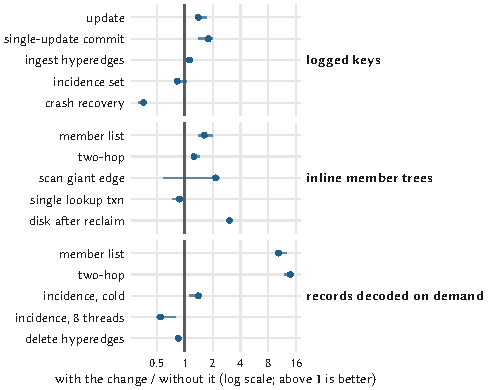
\includegraphics[width=\columnwidth]{figures/ablation}
\caption{Effect of three design choices, each measured on HStore alone at the commit that introduced it and at the commit before it. Logged keys and inline member trees run at scale~1, records decoded on demand at scale~4.}
\label{fig:ablation}
\end{figure}

To separate three of the decisions in \cref{sec:layout,sec:transactions}, we ran HStore alone at the commit that introduced each of them and at the commit just before it, with \M{ablrunslogical} runs of each build on the same machine (\cref{fig:ablation}). The two builds of a pair differ only in that change. Each pair comes from earlier in the project's history than the version measured above, so its absolute numbers are not comparable with \cref{tab:results}.

\paragraph{Logging keys instead of pages.} Before this change a commit wrote every new node from each changed leaf to the root. An update in a batch wrote \M{abllogicalwriteupdatewrittenbefore} before it and \M{abllogicalwriteupdatewrittenafter} after it, and a single-update commit \M{abllogicallatencycommitwrittenbefore} and \M{abllogicallatencycommitwrittenafter}. Batched updates became \M{abllogicalwriteupdate} times faster and single-update commits \M{abllogicallatencycommit} times faster. The cost is recovery. The open now replays the logged keys into the trees instead of finding pages already written, and opening the killed store took \M{abllogicalrecoverafter} instead of \M{abllogicalrecoverbefore}. The automatic checkpoint threshold, added later, bounds how much log the open has to replay. Most read workloads were 5 to 17\% slower after the change, two-hop queries excepted, and we have not investigated why.

\paragraph{Inline member trees.} Storing a small membership inside the hyperedge's record makes member lookups \M{ablinlinereadmembers} times faster and two-hop queries \M{ablinlinereadtwohop} times faster, because a lookup no longer follows a root reference to a tree of its own. It also removes a separate small leaf per hyperedge, and the files after reclamation shrink from \M{ablinlinediskcompactedbefore} to \M{ablinlinediskcompactedafter}. Single-lookup read transactions were slightly slower, at \M{ablinlinelatencyread} times their earlier rate.

\paragraph{Records decoded on demand.} With data larger than the cache, decoding a leaf record only when it is read makes member lookups \M{abllazyreadmembers} times faster (\M{abllazyreadmembersbefore} to \M{abllazyreadmembersafter} per second) and two-hop queries \M{abllazyreadtwohop} times faster, since a lookup that misses the cache decodes one record instead of a whole page. Incidence lookups right after a reopen gain \M{abllazyreadincidencecold} times. The same change cost almost half of the incidence rate from eight threads, from \M{abllazyreadincidenceparallelbefore} to \M{abllazyreadincidenceparallelafter} lookups per second, and deletes ran at \M{abllazychurndelete} times their earlier rate. We have not yet found what the eight readers contend on.

\subsection{Limits of this evaluation}

Both systems run on the JVM, on one machine, with one synthetic dataset. The dataset's skewed membership resembles real hypergraphs, but its hyperedges carry no properties beyond a name, and we did not test workloads with large property values or with many concurrent writers. HyperGraphDB is the only system we compare with, because it is the only embedded store we know of with first-class hyperedges, and its storage layer, JE~5.0.73, is more than a decade old. A comparison with a graph database storing reified hyperedges would answer a different question and is left for future work.

\section{Related work}
\label{sec:related}

\paragraph{Hypergraph and n-ary data stores.} HyperGraphDB~\cite{hgdb} is the closest system and our baseline. Its atoms are identified by UUID handles, a link is an ordered array of target handles, and an index maps every atom to its incidence set; storage is delegated to Berkeley DB Java Edition. A link is immutable, so changing a membership replaces the link, and the incidence index has to be updated for every member. OpenCog's AtomSpace~\cite{opencog} stores typed atoms and links in memory for reasoning workloads. TypeDB~\cite{typeql} gives $n$-ary relations and their role players a type system and a query language, and stores them in a key-value engine. Property-graph databases and RDF stores represent $n$-ary relations by reification~\cite{angles}, and Wikidata attaches qualifiers to statements for the same purpose~\cite{wikidata}. HStore differs from all of them in that a hyperedge's membership is a storage structure of its own, versioned, counted and summarised like every other tree in the engine.

\paragraph{Hypergraph processing.} Hygra~\cite{hygra}, MESH~\cite{mesh} and HyperX~\cite{hyperx} run analytics over hypergraphs held in memory, on one machine or a cluster. They assume a static input and optimise traversal and message passing. HStore is a storage engine for data that changes, and the analytic operators in its database layer read from its snapshots.

\paragraph{Copy-on-write and shadow paging.} Shadow paging goes back to Lorie~\cite{lorie}. Rodeh showed how to make B-trees copy-on-write with reference counts so that snapshots and clones are cheap~\cite{rodeh-shadowing}, and Btrfs builds a file system on that design~\cite{btrfs}. LMDB~\cite{lmdb} uses a copy-on-write B+tree with a single writer and readers that pin a root, much like HStore's generations. These systems write the changed path at every commit. HStore defers those writes to checkpoints and logs keys instead, which is closer to how a log-structured store absorbs small writes, while keeping the property that a published version never changes. Making data structures persistent in the functional sense~\cite{persistent} and the owner tokens that let one transaction change its own fresh nodes in place follow the same idea at the level of single objects.

\paragraph{Logging, recovery and log-structured storage.} ARIES~\cite{aries} logs page-level changes and redoes them in place. HStore never changes a page in place, so it logs logical key changes and replays them onto the last checkpoint's trees, and its only physical log records are page references for the rare commits that write pages. The rule that recovery stops at the first commit whose pages are missing addresses the reordering of writes by the file system that crash-consistency studies have catalogued~\cite{pillai,torturing}. Log-structured file systems~\cite{lfs} and LSM-trees~\cite{lsm} append all writes and reclaim space by cleaning or merging; Berkeley DB Java Edition, under HyperGraphDB, is a log-structured B+tree whose cleaner copies live records forward. HStore's compaction also copies live data forward, but because trees refer to pages by number through a directory, it copies pages without rewriting their parents. The Bw-tree~\cite{bwtree} uses a mapping table from logical page ids to physical addresses for a related reason, to install delta updates and relocate pages without changing references. LeanStore~\cite{leanstore} replaces the buffer pool's hash table with pointer swizzling; HStore's node cache stays a separate, budgeted table because its nodes are immutable and shared by every reader.

\paragraph{Order maintenance and set algebra.} Ordered hyperedges use the order-maintenance labelling of Dietz and Sleator and its later simplifications~\cite{dietz-sleator,bender-order}, as ORDPATH labels do for XML~\cite{ordpath}. Intersections use a leapfrog join~\cite{leapfrog}. Additive multiset hashes~\cite{multiset-hash} and polynomial fingerprints~\cite{karp-rabin} give each tree a content fingerprint that is independent of its shape.

\section{Conclusion}
\label{sec:conclusion}

HStore stores a hypergraph as trees of a single kind. Because every tree is a counted, summarized copy-on-write B+tree, the same code answers cardinality, rank, overlap and difference questions for a hyperedge's members, an atom's incidence set and the catalog, and the same checkpoint, recovery and compaction machinery serves all of them. Logging keys instead of pages removes most of the write cost that copy-on-write usually carries, and addressing pages through a directory lets compaction work without touching the trees. Against HyperGraphDB the result is faster reads and writes, fewer bytes written and less space on disk, at the price of more heap.

\paragraph{Limitations.} A database is opened by one process, and there is no replication. Commits are validated and appended to the log under one lock, so commit throughput is bounded by that short critical section even when writers change different trees. Retained history lives in memory, so after a restart time travel reaches back only to the last checkpoint and the commits replayed after it. Unwritten nodes and decoded nodes are both Java heap, and \cref{sec:eval-resources} shows that HStore keeps more of it than HyperGraphDB. At scale~4 the slowest single commit in a run is slower on HStore than on HyperGraphDB, and we have not yet found what causes these stalls. Decoding leaf records on demand roughly halved the rate of incidence lookups from eight threads at scale~4, a regression we have not yet traced either. For small databases most of the space left after deletes and compaction is the active log segment and the change feed rather than data pages, and their retention is not yet tuned for small stores.

\paragraph{Future work.} We plan to compare HStore with a graph database that stores reified hyperedges, to run the evaluation with data larger than main memory, and to measure many concurrent writers on overlapping hyperedges, where member-level conflict detection should matter most.

\begin{acks}
We thank Ujjwal Jain, who found that the first checkpoint after a recovery could record a log position that came before records recovery had discarded, so that a second crash would read them again, and contributed the fix together with the guard against reusing transaction ids described in \cref{sec:recovery}.
\end{acks}


\bibliographystyle{ACM-Reference-Format}
\bibliography{references}

\end{document}
